\documentclass[svgnames,t]{beamer}
\usepackage[english]{babel}
\usepackage{%
    fontspec,
    mathabx,
    pifont,
    etoolbox,
    listings,
    lstautogobble,
    tikz,
    multicol,
    moresize,
    relsize,
    array,
    booktabs,
    makecell
}

\setsansfont{Yanone Kaffeesatz}[
    UprightFont     = *-Regular ,
    BoldFont        = *-Bold ,
    BoldItalicFont  = *-Bold ,
    BoldSlantedFont = *-Bold ,
    ItalicFont      = *-Light ,
    SlantedFont     = *-Light ,
    SmallCapsFont   = *-Thin
]

%\setmonofont{Latin Modern Mono Prop}

\usetikzlibrary{
    overlay-beamer-styles,
    calc,
    positioning,
    decorations.pathreplacing,
    backgrounds, shadings,
    shapes
}

\tikzset{
    %Displaying keys
    onslide/.code args={<#1>#2}{\only<#1>{\pgfkeysalso{#2}}}, % \pgfkeysalso doesn't change the path
    scope on/.style={
        every node/.append style={visible on=#1},
        every path/.append style={visible on=#1}
    },
    %Path ending shapes
    to/.style={->,>=stealth},
    from/.style={<-,>=stealth},
    fromto/.style={<->,>=stealth},
    shorter/.style 2 args={shorten <= #1, shorten >= #2},
    %Hexagons
    hexagon/.style n args={3}{double arrow, double arrow head extend=0cm, inner sep=3pt, draw=#1, fill=#2, text=#3, thick},
    hexagon/.default={black}{gray!20}{black},
    hexagonOne/.style={hexagon={#1}{#1!30}{#1}},
    hexagonTwo/.style 2 args={hexagon={#1}{#1!#2}{#1}},
    hexagonThree/.style n args={3}{hexagon={#1}{#1!#2}{#3}},
    hexagonShade/.style n args={3}{double arrow, double arrow head extend=0cm, inner sep=3pt, thick, draw=#1, left color=#2, right color=#3},
    %General text element
    Shape/.style n args={3}{draw=#1, fill=#2, text=#3},
    genShape/.style 2 args={#1, inner sep=3pt, draw=#2, fill=#2!20, text=#2, thick},
    halo/.style={preaction={draw, #1, line width=7, -}},
}
%Colors for listings
\colorlet{background-color}{gray!20}
\colorlet{basic-color}{black}
\colorlet{keywords-color}{Goldenrod}
\colorlet{comment-color}{red!95!black}
\colorlet{strings-color}{ForestGreen}
\colorlet{builtins-color}{MediumBlue!90!black}
\colorlet{functions-color}{NavyBlue}
\colorlet{variables-color}{DarkOrange}
\colorlet{environment-color}{Gray}
\colorlet{external-color}{SteelBlue}

% https://tex.stackexchange.com/a/34000
\makeatletter
\lst@Key{countblanklines}{true}[t]%
    {\lstKV@SetIf{#1}\lst@ifcountblanklines}

\lst@AddToHook{OnEmptyLine}{%
    \lst@ifnumberblanklines\else%
       \lst@ifcountblanklines\else%
         \advance\c@lstnumber-\@ne\relax%
       \fi%
    \fi}
\makeatother

%listings set
\lstdefinestyle{MyBash}{
backgroundcolor=\color{background-color}, % choose the background color; you must add \usepackage{color} or \usepackage{xcolor}
breakatwhitespace=false,            % sets if automatic breaks should only happen at whitespace
breaklines=true,                    % sets automatic line breaking
captionpos=b,                       % sets the caption-position to bottom
deletekeywords={...},               % if you want to delete keywords from the given language
escapeinside={@|}{|@},              % if you want to add LaTeX within your code
extendedchars=true,                 % lets you use non-ASCII characters; for 8-bits encodings only,
                                    % does not work with UTF-8
frame=single,                       % adds a frame around the code
framerule=0pt,                      % Width of the frame rule
framesep=3pt,                       % separation around text
linewidth=\textwidth,               % defines the base line width for listings
xleftmargin=6mm,                    % Margin left
xrightmargin=6mm,                   % Margin right
numbers=left,                       % where to put the line-numbers; possible values are (none, left, right)
numberblanklines=false,             % suppress numbers on empty lines
countblanklines=false,              % NOT standard! Avoid counting empty lines: https://tex.stackexchange.com/a/34000
numbersep=8pt,                      % how far the line-numbers are from the code
numberstyle=\tiny\color{black},     % the style that is used for the line-numbers
rulecolor=\color{black},            % if not set, the frame-color may be changed on line-breaks within not-black text
                                    % (e.g. comments (green here))
showspaces=false,                   % show spaces everywhere adding particular underscores; it overrides 'showstringspaces'
showstringspaces=false,             % underline spaces within strings only
showtabs=false,                     % show tabs within strings adding particular underscores
stepnumber=1,                       % the step between two line-numbers. If it's 1, each line will be numbered
tabsize=2,                          % sets default tabsize to 2 spaces
title=\lstname,                     % show the filename of files included with \lstinputlisting; also try caption instead of title
%
%Base style for this presentation 
keepspaces=true,                    % keeps spaces in text, useful for keeping indentation of code
                                    % (possibly needs columns=flexible)
language=bash,
basicstyle=\ttfamily\scriptsize\color{basic-color},
keywordstyle=\color{keywords-color},
stringstyle=\color{strings-color},
commentstyle=\color{comment-color},
morestring=[b][\color{strings-color}]{"},
morestring=[d][\color{strings-color}]{'},
moredelim=[is][\color{basic-color}]{|+}{+|}, % I will use this for terminal output
literate={`}{\textasciigrave}1, % https://tex.stackexchange.com/a/466224/128737
literate={~}{{\textasciitilde}}1,
% literate=% literate={<replace>}{<replacement text>}{<width>}
%   {\#define}{{{\color{CarnationPink}\#define}}}{6}
%   {\#include}{{{\color{CarnationPink}\#include}}}{7},
alsoletter=0123456789![]/\{\}.:+, % This to mark the symbols in keyword/emph[5] to be highlighted (otherkeywords does not work i.e. it highlights also in comments!) -> manual at page 45
morekeywords={if, then, else, elif, fi, case, esac, for, select, while, until, do, done, in, function, time, [[, ]], \{, \}, !, coproc}, %https://askubuntu.com/a/513712
emph=[1]{CreateListOfFiles, LevelOne, LevelTwo, LevelThree, Test, SecondsToTimeStringWithDays, ExampleFunction,
         ExampleFunction_implementation, ExtractColumnFromFile, CalculateSizeOfFiles, ReportOnLargestDirectories,
         CountTill5From, FifthElementOf, CreateAuxiliaryFiles, CleanAuxiliaryFiles, Failure, FailureMsg, Simulation},
emphstyle=[1]{\color{functions-color}}, %Functions
emph=[2]{variableName, invisibleVariable, prefix, day, today, song, aVar, bVar, langRegex, deadline, now,
         index, file, fgbg, color, reference, files, array, message, entry, index, dict, key, flag, line, inputTime,
         days, hours, minutes, seconds, globalVar, pid, extglobSet, counter, filename, extension},
emphstyle=[2]{\color{variables-color}}, %Variables
emph=[4]{PATH, SHELL, IFS, BASH_ALIASES, BASH_REMATCH, PS3, REPLY, HOME, LANGUAGE, EDITOR, PIPESTATUS, PWD, FUNCNEST,
         DIRSTACK, PWD, OLDPWD, SHELLOPTS, BASHOPTS, TIMEFORMAT, COMP_CWORD, COMP_LINE, COMP_POINT, COMP_TYPE, COMP_KEY,
         COMP_WORDBREAKS, COMP_WORDS, COMPREPLY, INPUTRC},
emphstyle=[4]{\color{environment-color}}, %Environment variables
emph=[5]{alias, bg, bind, break, builtin, cd, command, compgen, complete, continue, declare, dirs, disown, echo, enable, eval,
         exec, exit, export, false, fc, fg, getopts, hash, help, history, jobs, kill, let, local, logout, popd, printf, pushd, pwd,
         read, readonly, return, set, shift, shopt, source, suspend, test, times, trap, true, type, typeset, ulimit, umask,
         % case, if, until, while  % <--- these built-in are keywords and I leave them highlighted as such
         unalias, unset, wait, :, ., [, ]},
emphstyle=[5]{\color{builtins-color}}, %Shell built-in
emph=[6]{man, apropos, ls, rm, g++, chmod, cp, awk, sed, cut, perl, args, date, grep, sleep, tput, seq, cat, wc, sort, tail,
         head, sdiff, tar, mktemp, mkdir, ps, emacs, systemd, timeout, parallel, xargs, gnuplot, pdflatex, vi, ping, bash,
         egrep, shuf, stat, find, fgrep, bc, tr, paste, expr, diff, touch},
emphstyle=[6]{\color{external-color}}, %(External) commands
emph=[7]{},
emphstyle=[7]{\color{variables-color}}, %Class for local variables (usually with bad names)
emph=[8]{},
emphstyle=[8]{\color{builtins-color}}, %Class for local commands (usually with bad names)
%
%Additional customizations
belowskip=-7mm,
aboveskip=3pt,
autogobble=true, % lstautogobble needed!
}

\lstnewenvironment{Bash}[1][] %I will rarely use this because putting a $ in it as prompt breaks down TeXclipse highlight syntax!
    {\lstset{style=MyBash, #1}}
    {}

\def\bash{\lstinline[style=MyBash, basicstyle=\ttfamily\color{black}]}

%This additional style is to just print odd numbers (NOTE: style keyword can be repeated and it is cumulative!)
\lstdefinestyle{oddnumbers}{
    stepnumber=2,
    firstnumber=0,
    numberstyle={\tiny\color{black}\ifodd\value{lstnumber}\relax\else\refstepcounter{lstnumber}\fi\tiny\color{black}\ifodd\value{lstnumber}\relax\else\refstepcounter{lstnumber}\fi}
}

%This additional style is to just print odd numbers (NOTE: style keyword can be repeated and it is cumulative!)
\lstdefinestyle{smaller}{
    basicstyle={\linespread{1.2}\ttfamily\ssmall\color{basic-color}}
}

\newcommand<>{\tc}[2]{\textcolor#3{#1}{#2}}
\newcommand{\tikzmark}[1]{\tikz[overlay,remember picture, baseline=-0.5ex] \node at (0,0) (#1) {};}
\newcommand{\URLsymbol}[2][white]{%
    \begin{tikzpicture}[every path/.style={line width=3, rounded corners, #2}]
        \pgfmathsetmacro{\longSide}{0.9}
        \pgfmathsetmacro{\shortSide}{0.3}
        \draw[rotate=45, xshift=0.5*\longSide cm]       (0,0) rectangle (\longSide, \shortSide);
        \draw[rotate=45, halo=#1, #2!50]                   (0,0) rectangle (\longSide, \shortSide);
        \draw[rotate=45, halo=#1, xshift=0.5*\longSide cm] (0, 0.5*\shortSide) -- (0,0) -- (\longSide, 0) -- (\longSide, 0.5*\shortSide);
    \end{tikzpicture}
}
\NewDocumentCommand{\URL}{ O{black} m m O{BGLIGHT} }%
{%
    \raisebox{-0.4ex}{\resizebox{!}{2ex}{\URLsymbol[#4]{#1}}}{\href{#2}{\textcolor{#1}{#3}}}
}

\NewDocumentCommand{\addSection}{ m O{} m m }%
{%
    \setbeamertemplate{section page}[Iceland][#2]{#3}{#4}
    \section{#1}
}

\makeatletter
\newcommand*\keystroke[1]
{%
    \begin{tikzpicture}[baseline=($(key.base)!0.8!(key.south)$), very thin]%
        \pgfmathsetlengthmacro{\textHeight}{0.9*\f@size}
        \pgfmathsetlengthmacro{\textHeightPlus}{1.25*\textHeight}
        \pgfmathsetlengthmacro{\roundedSmall}{0.2}
        \pgfmathsetlengthmacro{\roundedLarge}{0.4}
        \pgfmathsetlengthmacro{\dl}{0.5\pgflinewidth}
        \node[font=\sffamily, inner xsep=2pt, inner ysep=1pt] (text) {\scalebox{1.2}[0.75]{\textsmaller[2]{#1\strut}}};
        \node[rounded corners=\roundedLarge, minimum size=\textHeight, anchor=north west] (key) at (text.north west){};
        \node[rounded corners=\roundedSmall, minimum size=\textHeightPlus] (frame) at ($(key.center)!0.05!(key.south)$){};
        \path coordinate (keyNW) at ($(key.north west)+(\roundedLarge,-\dl)$)
              coordinate (keyNE) at ($(key.north east)-(\roundedLarge,+\dl)$)
              coordinate (keyEN) at ($(key.north east)-(-\dl,\roundedLarge)$)
              coordinate (keyES) at ($(key.south east)+(+\dl,\roundedLarge)$)
              coordinate (keySE) at ($(key.south east)-(\roundedLarge,+\dl)$)
              coordinate (keySW) at ($(key.south west)+(\roundedLarge,-\dl)$)
              coordinate (keyWS) at ($(key.south west)+(+\dl,\roundedLarge)$)
              coordinate (keyWN) at ($(key.north west)-(-\dl,\roundedLarge)$)
              coordinate (frameNW) at ($(frame.north west)+(\roundedSmall,-\dl)$)
              coordinate (frameNE) at ($(frame.north east)-(\roundedSmall,+\dl)$)
              coordinate (frameEN) at ($(frame.north east)-(+\dl,\roundedSmall)$)
              coordinate (frameES) at ($(frame.south east)+(-\dl,\roundedSmall)$)
              coordinate (frameSE) at ($(frame.south east)-(\roundedSmall,-\dl)$)
              coordinate (frameSW) at ($(frame.south west)+(\roundedSmall,+\dl)$)
              coordinate (frameWS) at ($(frame.south west)+(+\dl,\roundedSmall)$)
              coordinate (frameWN) at ($(frame.north west)-(-\dl,\roundedSmall)$);
        \foreach \n in {NW,NE,EN,ES,SE,SW,WS,WN}{
            \draw[line cap=round, ultra thin] (key\n) -- (frame\n);
        }
        \begin{scope}[on background layer]
            \node[draw, rounded corners=\roundedSmall, minimum size=\textHeightPlus, fill=fg] at ($(key.center)!0.05!(key.south)$){};
            \node[draw, rounded corners=\roundedLarge, lower right=gray!20, lower left=gray!50, upper right=gray!50, upper left=gray!80, minimum size=\textHeight, anchor=north west] at (text.north west){};
            \fill [gray!70!bg] (keyNW) -- (keyNE) -- (frameNE) -- (frameNW) -- cycle;
            \fill [gray!50!bg] (keyWS) -- (keyWN) -- (frameWN) -- (frameWS) -- cycle;
            \fill [gray!30!bg] (keyES) -- (keyEN) -- (frameEN) -- (frameES) -- cycle;
            \fill [gray!10!bg]  (keySW) -- (keySE) -- (frameSE) -- (frameSW) -- cycle;
        \end{scope}
  \end{tikzpicture}%
}
\makeatother

\newcommand{\Remark}[2][1mm]
{%
    \hspace{#1}{\tiny\{~#2~\}}%
}

\newcommand{\FrameRemark}[2][1-]%
{%
    \begin{tikzpicture}[remember picture, overlay]
        \node[font=\tiny, anchor=south, visible on=<#1>] at (current page.south) {#2};
    \end{tikzpicture}
}

\newcommand{\MakeEnumerateBox}[1]%
{%
    \hbox{%
      \usebeamerfont*{item projected}%
      \usebeamercolor[bg]{item projected}%
      \vrule width2.25ex height1.85ex depth.4ex%
      \hskip-2.25ex%
      \hbox to2.25ex{%
        \hfil%
        \color{fg}#1%
        \hfil}%
    }%
}

\renewcommand{\checkmark}[1][PS]{\tc{#1}{\ding{51}}}
\newcommand{\crossmark}[1][PT]{\tc{#1}{\ding{55}}}

\def\quizOverlay{1}
\newcounter{QuizNumber}
\resetcounteronoverlays{QuizNumber}% To avoid the counter being increased by overlays
\newenvironment{quiz}[2][1]{%
    \edef\tmpNumber{\numexpr #1 +1\relax}%
    \gdef\quizOverlay{\the\tmpNumber}%
    \stepcounter{QuizNumber}%
    \medskip%
    % mbox to avoid newline after hbox of enumerate
    \mbox{\MakeEnumerateBox{\theQuizNumber}}\enspace #2%
    \begin{itemize}%
}{%
    \end{itemize}%
    \bigskip%
}

\newcommand{\wrongChoice}[1]%
{%
    \item[\alt<\quizOverlay->{\crossmark}{$\bullet$}] #1
}

\newcommand{\correctChoice}[1]%
{%
    \item[\alt<\quizOverlay->{\checkmark}{$\bullet$}] #1
}

\graphicspath{{Figures/}{Figures/Iceland/}}
\makeatletter
\newif\ifgraphicexist

\catcode`\*=11
\newcommand\IfImageCanBeIncluded[1]{% Taken from https://tex.stackexchange.com/a/567990/128737
    \begingroup
        \global\graphicexisttrue
        \ifx\detokenize\@undefined\else
            \edef\Gin@extensions{\detokenize\expandafter{\Gin@extensions}}%
        \fi
        \let\input@path\Ginput@path
        \expandafter\filename@parse\expandafter{#1}%
        \ifx\filename@ext\Gin@gzext
            \expandafter\filename@parse\expandafter{\filename@base}%
            \ifx\filename@ext\relax
                \let\filename@ext\Gin@gzext
            \else
                \edef\Gin@ext{\Gin@ext\Gin@sepdefault\Gin@gzext}%
            \fi
        \fi
        \ifx\filename@ext\relax
            \@for\Gin@temp:=\Gin@extensions\do{%
                \ifx\Gin@ext\relax
                    \Gin@getbase\Gin@temp
                \fi}%
        \else
            \Gin@getbase{\Gin@sepdefault\filename@ext}%
            \ifx\Gin@ext\relax
                \global\graphicexistfalse
                \let\Gin@savedbase\filename@base
                \let\Gin@savedext\filename@ext
                \edef\filename@base{\filename@base\Gin@sepdefault\filename@ext}%
                \let\filename@ext\relax
                \@for\Gin@temp:=\Gin@extensions\do{%
                    \ifx\Gin@ext\relax
                        \Gin@getbase\Gin@temp
                    \fi}%
                    \ifx\Gin@ext\relax
                        \let\filename@base\Gin@savedbase
                        \let\filename@ext\Gin@savedext
                    \fi
                \fi
                \ifx\Gin@ext\relax
                    \global\graphicexistfalse
                    \def\Gin@base{\filename@area\filename@base}%
                    \edef\Gin@ext{\Gin@sepdefault\filename@ext}%
                \fi
        \fi
        \ifx\Gin@ext\relax
            \global\graphicexistfalse
        \else
        \@ifundefined{Gin@rule@\Gin@ext}%
            {\global\graphicexistfalse}%
            {}%
        \fi
        \ifx\Gin@ext\relax 
            \gdef\imageextension{unknown}%
        \else
            \xdef\imageextension{\Gin@ext}%
        \fi 
    \endgroup 
    \ifgraphicexist
        \expandafter \@firstoftwo
    \else
        \expandafter \@secondoftwo
    \fi
}
\catcode`\*=12
\makeatother

% Compile with or without photos
\newif\ifCompileWithPhotos
\CompileWithPhotostrue

% Compile with or without photos
\newif\ifAddLinkToTOC
\AddLinkToTOCtrue

\mode<presentation>
{
    \usetheme{Relax}
    \defbeamertemplate{footline}{Empty}{}
    \setbeamersize{text margin left=8mm,text margin right=8mm}
    %\setbeamerfont{section title}{size=\Huge}
    \defbeamertemplate*{section page}{Iceland}[3][]
    {
        \begin{tikzpicture}[overlay,remember picture, every node/.style={inner sep=0pt}]
            \usebeamercolor{section page background canvas}
            \fill[bg] (current page.south west) rectangle (current page.north east);
            \node[text depth=0.5ex, anchor=west] () (sectionTitle) at ($(current page.north west)+(5mm,-8mm)$)
                  {\usebeamerfont{section title}\usebeamercolor[fg]{section title}\insertsectionhead};
            \node[anchor=north east, inner sep=0] (plan) at ($(current page.north east)-(1mm,1mm)$) {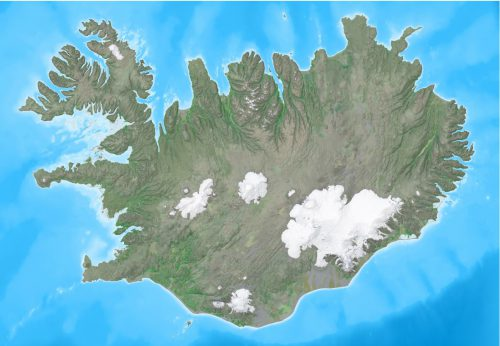
\includegraphics[width=0.21\textwidth, clip, trim=0 0 0 1mm]{Map}};
            \node[anchor=north] (photo) at ($(plan.south west)!0.5!(sectionTitle.south west |- plan.south)-(0,1mm)$) {
                \ifCompileWithPhotos%
                    \IfImageCanBeIncluded{#2}{%
                        \includegraphics[width=0.85\textwidth]{#2}
                    }{%
                        \includegraphics[width=0.75\textwidth]{example-image-a}
                    }
                \else
                    \includegraphics[width=0.75\textwidth]{example-image-a}
                \fi
            };
            \node[text depth=0.5ex, below = 2mm of photo.south east, anchor=north east, xshift=-2pt]{#3};
            \ifthenelse{\isempty{#1}}{}%
            {
                \begin{scope}[x={($ (plan.south east) - (plan.south west) $ )},y={( $ (plan.north west) - (plan.south west)$ )}, shift={(plan.south west)}]
                    %\draw[help lines,xstep=.1,ystep=.1] (0,0) grid (1,1);
                    \node[anchor=south, inner sep=0] at (#1) {
\includegraphics[width=2mm]{Pin}};
                \end{scope}
            }
            \ifCompileWithPhotos
                \IfImageCanBeIncluded{#2}{%
                    \node[rotate=90, anchor=west, font=\ssmall] at ($(current page.south east)+(-2mm,1mm)$) {{\raisebox{-2mm}{\Large\textcopyright}} Photo: All rights are reserved};
                }{}
            \fi
        \end{tikzpicture}
    }
    %Add a link to table of content on frames with a footline
    \addtobeamertemplate{footline}{}{%
        \ifAddLinkToTOC%
            \begin{tikzpicture}[remember picture,overlay]
                %xelatex needs \XeTeXLinkBox, won't create a link unless it
                %finds text --- rules don't work without \XeTeXLinkBox.
                %Still builds correctly with pdflatex and lualatex
                \node[anchor=south east, inner sep=2pt] at (current page.south east) {\hyperlink{toc}{\XeTeXLinkBox{
\includegraphics[width=3mm]{TOC}}}};
            \end{tikzpicture}%
        \fi%
    }%
}

\makeatletter
\AtBeginSection[]% <- Empty optional argument, do nothing for \section*
{%
    \ifnum\beamer@tocsectionnumber>0%
        \begin{frame}[plain, noframenumbering]{}
             \sectionpage
        \end{frame}
    \fi
}
\makeatother

%Append code to put third CSC logo on titlepage
\appto\titlepage{%
    \begin{tikzpicture}[remember picture, overlay]
        \node[anchor=south] at (current page.south) {
\includegraphics[width=25mm]{LogoCSC}};
    \end{tikzpicture}
}

%===============================================================%
\title{Introduction to Bash scripting language}
\author{Alessandro Sciarra \texorpdfstring{\\}{} {\tiny Z02~--~Software Development Center}}
\institute{Organised by the CSC Frankfurt}
\titlegraphic{
\includegraphics[width=20mm]{LogoCRC}}
\titlepagelogo{
\includegraphics[width=20mm]{LogoGoethe}}
%===============================================================%


%===================%
\subtitle{Day 2}
\date{27.10.2020}
%===================%

\begin{document}
    %-------------------------------%
%  Author: Alessandro Sciarra   %
%    Date: 4 Jul 2019           %
%-------------------------------%

%~~~~~~~~~~~~~~~~~~~~~~~~~~~~~~~~~~~~~~~~~~~~%
\begin{frame}[plain,noframenumbering]
    \titlepage
\end{frame}
%~~~~~~~~~~~~~~~~~~~~~~~~~~~~~~~~~~~~~~~~~~~~%
\begin{frame}[plain,noframenumbering]{Topics of the day}
    \medskip
    \begin{columns}[t]
        \begin{column}{.45\textwidth}
            \hspace*{4mm}
            \begin{minipage}[t][0.45\textheight]{\textwidth}
                \tableofcontents[sections={1-4}]
            \end{minipage}
        \end{column}
        \begin{column}{.45\textwidth}
            \begin{minipage}[t][0.45\textheight]{\textwidth}
                \tableofcontents[sections={5-}]
            \end{minipage}
        \end{column}
    \end{columns}
    \vspace{6mm}
    \begin{varblock}{example}[0.9\textwidth]{You know already the basics}
        Although only one third of the course is over, you learnt already almost everything about the core of Bash.
        Today we will complete \,\textasciitilde90\% of the picture.
    \end{varblock}
\end{frame}
%~~~~~~~~~~~~~~~~~~~~~~~~~~~~~~~~~~~~~~~~~~~~%

    \addSection{Conditional blocks}[0.175,0.2]{EuroAsiaticPlates}{The bridge between two continents}
    %-------------------------------%
%  Author: Alessandro Sciarra   %
%    Date: 23 Sep 2020          %
%-------------------------------%

%~~~~~~~~~~~~~~~~~~~~~~~~~~~~~~~~~~~~~~~~~~~~%
\begin{frame}{Exit code}
    \vspace{-3mm}
    Every command in Bash terminates with an exit code:
    \begin{description}
        \item[\texttt{\$?}]
            Shows the exit code of the last foreground process that terminated\\
            It is a 8-bit integer $\;$\texttt{\$?}${}\in{}$\texttt{\{0,\dots,255\}} \hfill\Remark{Indeed, only the least significant 8 bits count}
        \item[\texttt{0}] Denotes success
        \item[$\neq$\texttt{0}] Denotes failure, in general the meaning is up to the command
        \item[\texttt{1}] Miscellaneous errors
        \item[\texttt{2}] Misuse of shell builtins
        \item[\texttt{126}] Command invoked cannot execute
        \item[\texttt{127}] \PP{\texttt{"}command not found\texttt{"}} error
        \item[\texttt{128}] Invalid argument to exit
        \item[\texttt{128 + n}] Fatal error signal \texttt{"n"} \Remark{For example, \PB{\texttt{130}} means that the script terminated by Control-C}
    \end{description}
    \begin{varblock}{alerted}[0.45\textwidth]{Which exit code should I use?}
        \PQ{Avoid reserved one, be consistent!}
    \end{varblock}
\end{frame}
%~~~~~~~~~~~~~~~~~~~~~~~~~~~~~~~~~~~~~~~~~~~~%
\begin{frame}[fragile]{The \bash|if| keyword}
    \vspace{-3mm}
    \begin{itemize}
        \item Since it is a keyword, it requires a precise syntax (not a surprise)
        \item It executes a command (or a set of commands) and checks that command's exit code to see whether it was successful
        \item Different layouts possible, choose a readable one!
    \end{itemize}

    \begin{lstlisting}[style=MyBash, numbers=none]
        if@|\textvisiblespace|@COMMAND
        then
            # COMMAND's exit code was 0
        else
            # COMMAND's exit code was different from 0
        fi

        if@|\textvisiblespace|@COMMAND; then
            # COMMAND's exit code was 0
        elif@|\textvisiblespace|@ANOTHER_COMMAND; then
            # ANOTHER_COMMAND's exit code was 0
        else
            # ANOTHER_COMMAND's exit code was different from 0
        fi
    \end{lstlisting}
\end{frame}
%~~~~~~~~~~~~~~~~~~~~~~~~~~~~~~~~~~~~~~~~~~~~%
\begin{frame}[fragile]{The command in a conditional block}
    \vspace{-1mm}
    \begin{itemize}
        \setlength{\itemsep}{2mm}
        \item In principle it can be any command
        \item There are specifically designed commands to test things:\\[0.5em]
                \begin{tabular}{>{\ttfamily\color{PB}}rl}
                    \makecell[rt]{test \\ \tc{fg}{\sffamily or} [} &
                    \makecell[lt]{A normal command that reads its arguments and does \\
                                  some checks with them. The \bash{[} variant requires a \texttt{]} as last argument.}\\[2em]
                    \makecell[rt]{\tc{keywords-color}{[[}} &
                    \makecell[lt]{A special shell keyword that offers more versatility\\
                                  like \PP{pattern matching} and \PP{regex support}} \\
                \end{tabular}
        \item Multiple commands can be concatenated using control operators \texttt{\&\&} and \texttt{||}
    \end{itemize}
    \begin{varblock}{}[0.9\textwidth]{Which syntax should I prefer?}
        Whenever you are making a \textbf{Bash} script, you should always use \texttt{\tc{keywords-color}{[[}} rather than \bash{[}.\\
        If portability is an issue, e.g.\ you are writing a \textbf{sh}ell script, \\ you should use \bash{[}, because it is far more portable.
    \end{varblock}
\end{frame}
%~~~~~~~~~~~~~~~~~~~~~~~~~~~~~~~~~~~~~~~~~~~~%
\begin{frame}[fragile]{The \bash|test| command and its friend \bash{[}}
    \vspace{-4mm}
    \begin{center}
        \begin{minipage}{0.85\textwidth}
            \begin{description}[<only@1>][\texttt{-v VARIABLE}]
                \item[\texttt{-e FILE}] True if file exists
                \item[\texttt{-f FILE}] True if file is a regular file (not a directory or device file)
                \item[\texttt{-d FILE}] True if file is a directory
                \item[\texttt{-s FILE}] True if file exists and is not empty
                \item[\texttt{-z STRING}] True if the string is empty (it's length is zero)
                \item[\texttt{-n STRING}] True if the string is not empty (it's length is not zero)
                \item[\texttt{-v VARIABLE}] True if the shell variable is set (has been assigned a value)$^\star$
            \end{description}
        \end{minipage}
        \begin{minipage}{0.9\textwidth}
            \begin{description}[<only@2>][\texttt{STRING != STRING}]
                \item[\texttt{STRING  = STRING}] True if the first string is identical to the second
                \item[\texttt{STRING != STRING}] True if the first string is not identical to the second
                \item[\texttt{STRING \textbackslash< STRING}] True if the first string sorts before the second
                \item[\texttt{STRING \textbackslash> STRING}] True if the first string sorts after the second
                \item[\texttt{! EXPR}] Inverts the result of the expression (logical NOT)
            \end{description}
        \end{minipage}
        \begin{minipage}{0.9\textwidth}
            \begin{description}[<only@3>][\texttt{INT -eq INT}]
                \item[\texttt{INT -eq INT}] True if both integers are identical
                \item[\texttt{INT -ne INT}] True if the integers are not identical
                \item[\texttt{INT -lt INT}] True if the first integer is less than the second
                \item[\texttt{INT -gt INT}] True if the first integer is greater than the second
                \item[\texttt{INT -le INT}] True if the first integer is less than or equal to the second
                \item[\texttt{INT -ge INT}] True if the first integer is greater than or equal to the second
            \end{description}
        \end{minipage}
    \end{center}
    \begin{onlyenv}<1>
        \begin{lstlisting}[style=MyBash, style=oddnumbers, xleftmargin=10mm, xrightmargin=10mm, aboveskip=2mm]
            $ ls -d */
            |+TeX+|
            $ if [ -d 'TeX' ]; then echo 'YES'; else echo 'NO'; fi
            |+YES+|
            $ if [ -e 'TeX' ]; then echo 'YES'; else echo 'NO'; fi
            |+YES+|
            $ if [ -s 'TeX' ]; then echo 'YES'; else echo 'NO'; fi
            |+YES+|
            $ if [ -f 'TeX' ]; then echo 'YES'; else echo 'NO'; fi
            |+NO+|
        \end{lstlisting}
    \end{onlyenv}
    \begin{onlyenv}<2>
        \begin{lstlisting}[style=MyBash, style=oddnumbers, xleftmargin=-1mm, xrightmargin=-2mm, aboveskip=2mm]
            $ aVar="Kal El"
            $ bVar="Clark Kent"
            $ [ ${aVar} = ${aVar} ]
            bash: [: too many arguments
            $ if [ "${aVar}" = "${aVar}" ]; then echo 'YES'; else echo 'NO'; fi
            |+YES+|
            $ if [ "${aVar}" \> "${bVar}" ]; then echo 'YES'; else echo 'NO'; fi
            |+YES+|
            $ if [ 319 \< 7 ]; then echo 'YES'; else echo 'NO'; fi
            |+YES+| # 319 is < than 7 but it is not less than 7...
            $ unset aVar bVar
        \end{lstlisting}
    \end{onlyenv}
    \begin{onlyenv}<3>
        \begin{lstlisting}[style=MyBash, style=oddnumbers, xleftmargin=8mm, xrightmargin=8mm, aboveskip=2mm]
            $ if [ 319 -lt 7 ]; then echo 'YES'; else echo 'NO'; fi
            |+NO+|
            $ if [ 7 -ne 7 ]; then echo 'YES'; else echo 'NO'; fi
            |+NO+|
            $ if [ 7 -eq 7 ]; then echo 'YES'; else echo 'NO'; fi
            |+YES+|
            $ if [ 7 -gt 7 ]; then echo 'YES'; else echo 'NO'; fi
            |+NO+|
            $ if [ 7 -ge 7 ]; then echo 'YES'; else echo 'NO'; fi
            |+YES+|
        \end{lstlisting}
    \end{onlyenv}
    \begin{tikzpicture}[remember picture, overlay]
        \node[anchor=north east, font=\scriptsize, visible on=<1>] at ($(current page.north east)-(1mm,1mm)$) {$^\star$\PB{Since Bash v4.2}};
    \end{tikzpicture}
    \PrepareURLsymbol[PB]
    \FrameRemark{Many more tests are supported $\to$ for a complete list refer to the \URL*{https://www.gnu.org/software/bash/manual/}{Bash manual v5.2 (section 6.4).}}
\end{frame}
%~~~~~~~~~~~~~~~~~~~~~~~~~~~~~~~~~~~~~~~~~~~~%
\begin{frame}[fragile]{The \bash{[[} keyword}
    \vspace{-2mm}
    \begin{itemize}[<only@1>]
        \item It supports the tests supported by the \bash{test} and \bash{[} commands$^{\star}$
        \item String equality (\texttt{=} or \texttt{==}) and inequality (\texttt{!=}) comparison is changed to \alert{pattern matching} by default.
              \PQ{\textbf{Patterns must be on the right hand side of the (in)equality.}}
              Each quoted part of the pattern is matched literally.
        \item \alert{It does not allow word-splitting} of its arguments!
        \item However, be aware that simple strings still have to be quoted properly
        \item Few more additional tests supported:
              \begin{description}[\texttt{STRING =\textasciitilde\ REGEX}]
                \item[\texttt{STRING =\textasciitilde\ REGEX}] True if the string matches the regex pattern
                \item[\texttt{( EXPR )}] Parentheses can be used to change the evaluation precedence
                \item[\texttt{EXPR \&\& EXPR}] True if both expressions are true (logical AND)\\[-0.5em] \Remark[0pt]{it does not evaluate the second expression if the first already turns out to be false}
                \item[\texttt{EXPR || EXPR}] True if either expression is true (logical OR) \\[-0.5em] \Remark[0pt]{it does not evaluate the second expression if the first already turns out to be true}
              \end{description}
        \item The alphabetically sorted test operators (\texttt{<} and \texttt{>}) do not need to be escaped
    \end{itemize}
    \begin{onlyenv}<2>
        \begin{lstlisting}[style=MyBash, aboveskip=-1mm, style=oddnumbers, style=smaller, xleftmargin=1mm, xrightmargin=1mm]
            $ aVar="Day_1.tex"; bVar='Hello world'
            # Pattern matching VS string comparison
            $ if [[ ${aVar} = *.tex ]]; then echo 'YES'; else echo 'NO'; fi
            |+YES+|
            $ if [[ *.tex = ${aVar} ]]; then echo 'YES'; else echo 'NO'; fi
            |+NO+|
            $ if [[ ${aVar} = "*.tex" ]]; then echo 'YES'; else echo 'NO'; fi
            |+NO+|
            $ if [[ ${aVar} = Day_?.tex && ${bVar} = [hH]* ]]; then echo 'YES'; else echo 'NO'; fi
            |+YES+|
            # Simple strings still have to be quoted properly!
            $ if [[ ${bVar} = Hello world ]]; then echo 'YES'; else echo 'NO'; fi
            |+bash: syntax error in conditional expression
            bash: syntax error near `world'+|
            $ if [[ ${bVar} = 'Hello world' ]]; then echo 'YES'; else echo 'NO'; fi
            |+YES+| # No word splitting occurred!
            $ if [[ ${emptyVar} = '' ]]; then echo 'YES'; else echo 'NO'; fi
            |+YES+|
            $ if [ ${emptyVar} = '' ]; then echo 'YES'; else echo 'NO'; fi
            |+bash: [: =: unary operator expected+|
            |+NO+|
            # Quotes necessary to use test [ command to check for empty variables
            $ if [ "${emptyVar}" = '' ]; then echo 'YES'; else echo 'NO'; fi
            |+YES+|
            $ unset aVar bVar
        \end{lstlisting}
    \end{onlyenv}
    \FrameRemark{$^{\star}$ Except \PB{\texttt{~EXPR -a EXPR~}} and \PB{\texttt{~EXPR -o EXPR~}} which should in any case not be used!}
\end{frame}
%~~~~~~~~~~~~~~~~~~~~~~~~~~~~~~~~~~~~~~~~~~~~%
\begin{frame}[fragile]{Control operators}
    \begin{overlayarea}{\textwidth}{0.56\textheight}
        \begin{description}[<only@1>][\texttt{\&\&}]
            \setlength{\itemsep}{5mm}
            \item[\texttt{\&\&}]
                 Used to build AND lists: Run one command only if another exited successfully
                 \begin{lstlisting}[style=MyBash, numbers=none, aboveskip=2mm]
                     COMMAND_1 && COMMAND_2
                     # Equivalent to
                     if COMMAND_1; then COMMAND_2; fi
                 \end{lstlisting}
            \item[\texttt{||}]
                 Used to build OR lists: Run one command only if another exited unsuccessfully
                 \begin{lstlisting}[style=MyBash, numbers=none, aboveskip=2mm]
                     COMMAND_1 || COMMAND_2
                     # Equivalent to
                     if ! COMMAND_1; then COMMAND_2; fi
                 \end{lstlisting}
        \end{description}
        \begin{onlyenv}<2-3>
            \begin{lstlisting}[style=MyBash, numbers=none, belowskip=-5mm]
                # The use of control operators is handy in simple cases
                [[ ${PATH} ]] && echo 'PATH variable set and non empty!'
                # Mostly they are used in script
                rm file || echo 'Could not delete file!'
                mkdir TeX && cd TeX
                source AuxiliaryOps.bash || exit 1
                # Avoid complicated one-liners which might easily be wrong!
                grep -q goodword "${file}" && ! grep -q badword "${file}" && rm "${file}" || echo "Couldn't delete: ${file}"
            \end{lstlisting}
            \centerline{\small\PQ{What happens if the first \bash{grep} fails (sets the exit status to 1)?}}
            \begin{uncoverenv}<3>
                \begin{lstlisting}[style=MyBash, numbers=none, aboveskip=3mm]
                    grep -q goodword "${file}" && ! grep -q badword "${file}" && { rm "${file}" || echo "Couldn't delete: ${file}"; }
                \end{lstlisting}
            \end{uncoverenv}
        \end{onlyenv}
    \end{overlayarea}
    \begin{varblock}{alerted}[0.8\textwidth]{Do not get overzealous with conditional operators}
        They can make your script hard to understand and sometimes you need fancy grouping to get your logic right!
    \end{varblock}
\end{frame}
%~~~~~~~~~~~~~~~~~~~~~~~~~~~~~~~~~~~~~~~~~~~~%
\begin{frame}[fragile]{Regular expressions in Bash}
    \begin{itemize}[<only@1>]
        \item Regular expressions are similar to Glob Patterns, but not for filename matching
        \item Since v3.0, Bash supports the \texttt{=\textasciitilde} operator to the \bash{[[} keyword
        \item This operator matches the string that comes before it against the regular expression pattern that follows it and it returns
              \begin{description}
                  \item[0] when the string matches the pattern
                  \item[1] If the string does not match the pattern
                  \item[2] In case the pattern's syntax is invalid
              \end{description}
        \item Bash uses the Extended Regular Expression dialect
              \begin{itemize}
                  \item[$\circ$] \URL[PS]{http://pubs.opengroup.org/onlinepubs/9699919799/basedefs/V1_chap09.html}{POSIX standard}
                  \item[$\circ$] \URL[PQ]{https://www.regular-expressions.info/posix.html}{The Premier website about Regular Expressions}
              \end{itemize}
        \item Regular Expression patterns that use capturing groups (parentheses) will have their captured strings assigned to the \bash|BASH_REMATCH| variable (array) for later retrieval
    \end{itemize}
    \begin{onlyenv}<2>
        \begin{lstlisting}[style=MyBash, style=oddnumbers, style=smaller]
            $ echo "${LANG}"
            |+en_GB.utf8+|
            $ langRegex='(..)_(..)'
            $ if [[ ${LANG} =~ ${langRegex} ]]
            > then
            >     echo "Your country code (ISO 3166-1-alpha-2) is ${BASH_REMATCH[2]}."
            >     echo "Your language code (ISO 639-1) is ${BASH_REMATCH[1]}."
            > else
            >     echo "Your locale was not recognised"
            > fi
            |+Your country code (ISO 3166-1-alpha-2) is GB.+|
            |+Your language code (ISO 639-1) is en.+|
        \end{lstlisting}
        \begin{varblock*}{}[0.9\textwidth]{General remarks}
            \begin{itemize}
                \item The best way to always be compatible is to put your regex in a variable and expand that variable in \bash{[[} without quotes, as we showed above.
                \item The pattern matching achieved by the \texttt{=} and \texttt{!=} operators can be achieved using regex: \alert{Find your way!}
            \end{itemize}
        \end{varblock*}
    \end{onlyenv}
    \FrameRemark<2>{The syntax \bash{"\$\{BASH\_REMATCH[1]\}"}, e.g.\ how to use an array variable, will be discussed in detail at a later point.}
\end{frame}












    \addSection{Loops}[0.73,0.3]{GlacierCave2}{Ice cave in the Breiðamerkurj\"okull}
    % 1. Rename all .jpeg into .jpg
% 2. Rename single spaces in filenames to underscores
% 3. Report of how many files per extension in present folder (loop to find extensions [just if with regex or grep instead of sort+uniq] , then loop over extensions to count them)
    \addSection{Choices}[0.655,0.255]{SkaftafellSvartifoss}{The Skaftafell natural park: Svartifoss}
    %-------------------------------%
%  Author: Alessandro Sciarra   %
%    Date: 8 Jul 2019           %
%-------------------------------%

%~~~~~~~~~~~~~~~~~~~~~~~~~~~~~~~~~~~~~~~~~~~~%
\begin{frame}[fragile]{The \,\bash|case|\, keyword}
    \vspace{-3mm}
    Completely equivalent to a \bash|if-elif-else-fi| construct, but often handy:
    \medskip
    \begin{lstlisting}[style=MyBash, numbers=none, belowskip=-5mm]
        case WORD in
            |+[ [(] pattern [| pattern]...) command-list ;;]...+|
        esac
    \end{lstlisting}
    \begin{overlayarea}{\textwidth}{\textheight}
        \begin{onlyenv}<1>
            \begin{itemize}
                \setlength{\itemsep}{0mm}
                \item The command-list corresponding to the first pattern that matches word is executed
                \item The match is performed according \PP{Pattern Matching} rules
                \item The \bash{|} is used to separate multiple patterns
                \item The \bash|)| operator terminates a pattern list
                \item A list of patterns and an associated command-list is known as a \textbf{clause}
            \end{itemize}
            \vspace{-5mm}
            \begin{center}
                \alert{\textbf{Before matching is attempted:}}\\[0.3em]
                \tikzmark{wordStart}tilde expansion\tikzmark{patternStart}\\
                parameter expansion\\
                command substitution\\
                arithmetic expansion\tikzmark{patternEnd}\\
                \tikzmark{wordEnd}quote removal
            \end{center}
        \end{onlyenv}
        \begin{tikzpicture}[remember picture, overlay, PP]
            \begin{scope}[scope on=<1>]
                \draw[very thick, decorate, decoration={brace,amplitude=6pt}] (patternStart -| patternEnd) ++(5mm,1mm) -- ($(patternEnd)+(5mm,-1mm)$)
                          node[midway, right=3mm, text width=18mm, align=center] {Pattern under-goes};
                \draw[very thick, decorate, decoration={brace,amplitude=6pt}] (wordEnd  -| wordStart) ++(-8mm,-1mm) -- ($(wordStart)+(-8mm,1mm)$)
                          node[midway, left=3mm, text width=18mm, align=center] {\texttt{WORD} under-goes};
            \end{scope}
        \end{tikzpicture}
        \begin{onlyenv}<2>
            \vspace{-3mm}
            \begin{lstlisting}[style=MyBash]
                case ${LANG} in
                    en* )
                        echo 'Hello!' ;;
                    fr* )
                        echo 'Salut!' ;;
                    de* )
                        echo 'Hallo!' ;;
                    it* )
                        echo 'Ciao!' ;;
                    es* )
                        echo 'Hola!' ;;
                    C | POSIX )
                        echo 'Hello World!' ;;
                    *)
                        echo 'I do not speak your language.' ;;
                esac
            \end{lstlisting}
        \end{onlyenv}
    \end{overlayarea}
    \FrameRemark{Using \bash|;&| or \bash|;;&| instead of \bash|;;| allows to execute the command list or to test the patterns of the next clause, respectively.}
\end{frame}
%~~~~~~~~~~~~~~~~~~~~~~~~~~~~~~~~~~~~~~~~~~~~%
\begin{frame}[fragile]{The \,\bash|select|\, keyword}
    \vspace{-3mm}
    A convenient statement for generating a menu of choices that the user can choose from:
    \medskip
    \begin{lstlisting}[style=MyBash, numbers=none, belowskip=-5mm]
        select NAME in WORDS; do
            # Body with commands -> break needed to terminate
        done
    \end{lstlisting}
    \begin{overlayarea}{\textwidth}{\textheight}
        \begin{onlyenv}<1>
            \begin{itemize}
                %\setlength{\itemsep}{0mm}
                \item The list of words following in is expanded, generating a list of items
                \item The set of expanded words is printed on the \alert{standard error}, each preceded by a number
                \item If the \bash|in WORDS| is omitted, the positional parameters are printed, as if \bash{in "$@"}
                \item The \bash|PS3| prompt is then displayed and a line is read from the standard input:
                      \begin{itemize}
                          \item[$\circ$] If the line consists of a number corresponding to one of the displayed words, then the value of \bash|NAME| is set to that word
                          \item[$\circ$] If the line is empty, the words and prompt are displayed again
                          \item[$\circ$] Any other value read causes \bash|NAME| to be set to null
                          \item[$\circ$] The line read is saved in the variable \bash|REPLY|
                      \end{itemize}
                \item It is good practice not to \bash|break| if the user typed something meaningless!
            \end{itemize}
        \end{onlyenv}
        \begin{onlyenv}<2>
            \begin{lstlisting}[style=MyBash]
                $ select file in *; do
                >     echo "You picked \"${file}\" (${REPLY})"
                >     break;
                > done
                |+1) Day_1.tex
                2) Day_2.tex
                3) Day_3.tex
                #? 2
                You picked "Day_2.tex" (3)+|
                $ echo "After select: \"${file}\" (${REPLY})"
                |+After select: "Day_2.tex" (2)+|
                $ unset file
            \end{lstlisting}
        \end{onlyenv}
        \begin{onlyenv}<3>
            \begin{lstlisting}[style=MyBash]
                $ select file in *; do
                >     echo "You picked \"${file}\" (${REPLY})"
                >     break;
                > done
                |+1) Day_1.tex
                2) Day_2.tex
                3) Day_3.tex
                #? dlfagfdsu
                You picked "" (dlfagfdsu)+|
                $ echo "After select: \"${file}\" (${REPLY})"
                |+After select: "" (dlfagfdsu)+|
                $ unset file
            \end{lstlisting}
        \end{onlyenv}
        \begin{onlyenv}<4>
            \begin{lstlisting}[style=MyBash]
                $ select file in *; do
                >     if [[ ${file} != '' ]]; then  # GOOD PRACTICE
                >         echo "You picked \"${file}\" (${REPLY})"
                >         break;
                >     fi
                > done; unset file
                |+1) Day_1.tex
                2) Day_2.tex
                3) Day_3.tex
                #? dlfagfdsu
                #? dgasdf
                #? 4
                #? 231345134
                #? 2
                You picked "Day_2.tex" (2)
            \end{lstlisting}
        \end{onlyenv}
    \end{overlayarea}
\end{frame}
%~~~~~~~~~~~~~~~~~~~~~~~~~~~~~~~~~~~~~~~~~~~~%





















    \addSection{Colours and cursor movements}[0.735,0.255]{JokursarlonBeach1}{Icebergs on the beach of the J\"okurs\'arl\'on}
    %-------------------------------%
%  Author: Alessandro Sciarra   %
%    Date: 11 Jul 2019          %
%-------------------------------%

%~~~~~~~~~~~~~~~~~~~~~~~~~~~~~~~~~~~~~~~~~~~~%
\begin{frame}{Colours and formatting in the terminal}{\URL[PB]{https://misc.flogisoft.com/bash/tip\_colors\_and\_formatting}{A good reference}}
    \vspace{-4mm}
    \begin{itemize}
        \item Most terminals are able to display colours and formatted texts thanks to \PP{escape sequences}
        \item Your script can benefit from using colours (e.g.\ \PQ{errors}, \alert{warnings}, \PS{info})
        \item You might run into compatibility problems (not really) {\scriptsize $\;$ \URL[PB]{https://misc.flogisoft.com/bash/tip\_colors\_and\_formatting\#terminals\_compatibility}{Compatibility list}}
        \item The \bash|echo| command has a \texttt{\alert{-e}} option to enable the parsing of the escape sequences
        \item The \bash|printf| command parses escape sequences
    \end{itemize}
    \vspace{-3mm}
    \begin{varblock}{}[0.35\textwidth]{Escape sequences}
        \texttt{<Esc>[\tc{red}{FormatCode}m}
    \end{varblock}
    \begin{itemize}
        \item The \texttt{<Esc>} character can be obtained with any of the following syntaxes:
              \begin{itemize}
                  \item[$\circ$] \texttt{\textbackslash{}e}
                  \item[$\circ$] \texttt{\textbackslash{}033}
                  \item[$\circ$] \texttt{\textbackslash{}x1B}
              \end{itemize}
        \item The \texttt{\tc{red}{FormatCode}} is an integer and different ones can be combined using semi-colons
    \end{itemize}
    \FrameRemark{The colors can vary depending of the terminal configuration!}
\end{frame}
%~~~~~~~~~~~~~~~~~~~~~~~~~~~~~~~~~~~~~~~~~~~~%
\begin{frame}[fragile]{Colours and format codes}
    \vspace{-4mm}
    \begin{onlyenv}<1>
        \begin{description}
            \setlength{\itemsep}{1pt}
            \item[0] Reset, all attributes off
            \item[1] Bold (or increased intensity)
            \item[2] Faint (decreased intensity)
            \item[3] Italic {\tiny \{~not widely supported, sometimes treated as inverse~\}}
            \item[4] Underline
            \item[5 or 6] Slow/Rapid Blink
            \item[7] Swap foreground and background colours
            \item[8] Hidden (useful for passwords)
            \item[2\{1..8\}] Reset second digit format (e.g.\ \PB{24} to stop underlining)$^\star$
            \item[30 to 37] Set foreground colour \tikzmark{8start}
            \item[40 to 47] Set background colour \tikzmark{8end}
            \item[38;5;\{0..255\}] Set foreground colour \tikzmark{256start}
            \item[48;5;\{0..255\}] Set background colour \tikzmark{256end}
            \item[90 to 97] Set bright foreground colour \tikzmark{16start}
            \item[100 to 107] Set bright background colour \tikzmark{16end}
        \end{description}
    \end{onlyenv}
    \begin{onlyenv}<2>
        \fboxsep1pt
        \begin{lstlisting}[style=MyBash, style=oddnumbers, xleftmargin=0mm, xrightmargin=0mm]
            $ echo "Default \e[31mRed\e[0m"
            |+Default \e[31mRed\e[0m+|
            $ echo -e "Default \e[31mRed\e[0m"
            |+Default+| @|\texttt{\tc{FireBrick}{Red}}|@
            $ echo -e "Default \e[91mLight Red\e[0m"
            |+Default+| @|\texttt{\tc{red}{Light Red}}|@
            $ echo -e "Default \e[46mCyan\e[0m"
            |+Default+| @|\texttt{\colorbox{Turquoise}{Cyan}}|@
            $ echo -e "Default \e[106mLight Cyan\e[0m"
            |+Default+| @|\texttt{\colorbox{Cyan}{Light Cyan}}|@
            $ echo -e "Default \e[1mBold\e[0m"
            |+Default+| @|\texttt{\textbf{Bold}}|@
            $ echo -e "Default \e[4mUnderlined\e[0m"
            |+Default+| @|\texttt{\underline{Underlined}}|@
            $ echo -e "Default \e[4m\e[91mUnderlined\e[0m"
            |+Default+| @|\texttt{\tc{red}{\underline{Underlined}}}|@
            $ echo -e "Default \e[4;91mUnderlined\e[0m"
            |+Default+| @|\texttt{\tc{red}{\underline{Underlined}}}|@
            $ printf "Default \e[4;91mUnderlined\e[24m still red\e[0m Default"
            |+Default+| @|\texttt{\tc{red}{\underline{Underlined} still red}}|@ |+Default+|
            $ echo -e "\e[40;38;5;82m Hello \e[30;48;5;82m World \e[0m"
            @|\texttt{\colorbox{black}{\tc{green}{~Hello~}}\colorbox{green}{\tc{black}{~World~}}}|@
        \end{lstlisting}
    \end{onlyenv}
    \begin{onlyenv}<3>
        \begin{lstlisting}[style=MyBash, xleftmargin=0mm, xrightmargin=0mm]
            $ for fgbg in 38; do  # 38 48 to get also background
            >     for color in {0..255}; do
            >         printf "\e[${fgbg};5;%sm  %3s  \e[0m" ${color} ${color}
            >         if [[ $(((color + 1) % 16)) -eq 0 ]]; then
            >             echo
            >         fi
            >     done
            >     echo
            > done
        \end{lstlisting}
        \bigskip
        \centerline{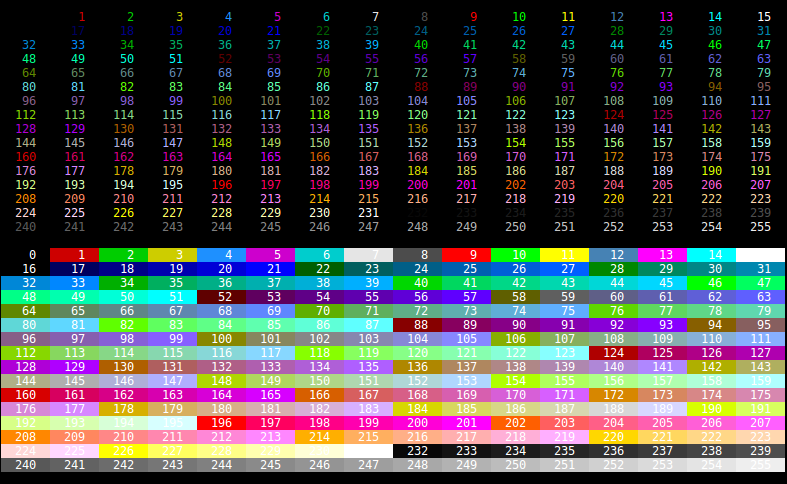
\includegraphics[width=0.95\textwidth, clip, trim=0 85mm 0 0]{ColoursTerminal}}
    \end{onlyenv}
    \begin{tikzpicture}[remember picture, overlay]
        \begin{scope}[scope on=<1>]
            \coordinate (yPos) at ($(8start)+(8mm,0mm)$);
            \foreach \n/\c in {8/PP, 16/PQ, 256/PS}{
                \draw[very thick, decorate, decoration={brace,amplitude=3pt}] (\n start -| yPos) ++(5mm,1mm) -- ($(\n end -| yPos)+(5mm,-1mm)$)
                      node[midway, right=2mm, text width=15mm, align=right, text=\c] {\n\ colours};
            }
            \node[anchor=north east, font=\ttfamily\large, rounded corners=1mm, draw=PP] at ($(current page.north east)-(8mm,4.5mm)$) {<Esc>[\tc{red}{FormatCode}m};
        \end{scope}
    \end{tikzpicture}
    \FrameRemark{$^\star$ GNOME Terminal 3.28 (VTE 0.52), debuting in Ubuntu 18.04 LTS, adds support for a \URL[PB]{https://askubuntu.com/a/985386}{few more styles}. Use code \PB{22} to unbold since \PB{21} is double underline!}
\end{frame}
%~~~~~~~~~~~~~~~~~~~~~~~~~~~~~~~~~~~~~~~~~~~~%
\begin{frame}[fragile]{Defining variables for colour codes}
    \vspace{-3mm}
    \begin{lstlisting}[style=MyBash, numbers=none]
        # Reset
        Default='\033[0m'
        # Regular Colors
        Black='\033[0;30m'
        Red='\033[0;31m'
        Green='\033[0;32m'
        Yellow='\033[0;33m'
        Blue='\033[0;34m'
        Magenta='\033[0;35m'
        Cyan='\033[0;36m'
        White='\033[0;37m'                 # Or you can wait to
        # Bold                             # learn about functions
        Bold='\033[1m'                     # and create your way!
        BBlack='\033[1;30m'
        BRed='\033[1;31m'
        BGreen='\033[1;32m'
        BYellow='\033[1;33m'
        BBlue='\033[1;34m'
        BMagenta='\033[1;35m'
        BCyan='\033[1;36m'
        BWhite='\033[1;37m'            # ...and so on and so forth!
    \end{lstlisting}
\end{frame}
%~~~~~~~~~~~~~~~~~~~~~~~~~~~~~~~~~~~~~~~~~~~~%
\begin{frame}[fragile]{Cursor movements}
    \vspace{-1mm}
    \begin{onlyenv}<1>
        In the same spirit of colours, the terminal cursor position can be moved:
        \smallskip
        \begin{description}[\texttt{<Esc><L>;<C>H}xxxxx]
            {\item[\texttt{<Esc>[<L>;<C>H}] Puts the cursor at line \texttt{L} and column \texttt{C}
            \item[\texttt{<Esc>[<L>;<C>f}] Puts the cursor at line \texttt{L} and column \texttt{C}
            \item[\texttt{<Esc>[<N>A}] Move the cursor up N lines
            \item[\texttt{<Esc>[<N>B}] Move the cursor down N lines
            \item[\texttt{<Esc>[<N>C}] Move the cursor forward N columns
            \item[\texttt{<Esc>[<N>D}] Move the cursor backward N columns
            \item[\texttt{<Esc>[2J}] Clear the screen, move to (0,0)
            \item[\texttt{<Esc>[K}] Erase to end of line
            \item[\texttt{<Esc>[s}] Save cursor position
            \item[\texttt{<Esc>[u}] Restore cursor position}
        \end{description}
    \end{onlyenv}
    \begin{onlyenv}<2>
        Use your imagination to take advantage of this functionality:
        \medskip
        \begin{lstlisting}[style=MyBash, numbers=none, xleftmargin=3mm, xrightmargin=3mm]
             $ while true; do
             >     printf "     $(date) \n\e[1A"
             >     sleep 1
             > done
             |+^C   Thu 11 Jul 18:07:26 CEST 2019+| # Stop it with CTRL-C
             
             # Here a crazy progress bar:
             $ while true; do
             >     printf '\e[s'
             >     printf '%0.s=' $(seq 1 $(bc -l <<< "$RANDOM/32767*100"))
             >     sleep 0.2
             >     printf '\e[u\e[K'  # Use \r instead of saving cursor
             > done
             |+======================^C+| # Stop it with CTRL-C
             
             $ printf 'You will never see my ${password}... MUAHAHA!\r\e[K'
             $
        \end{lstlisting}
    \end{onlyenv}
    \FrameRemark{The \bash|tput| command is a kind of wrapper for everything we learn in this section \,$\to$\,\URL[PB]{https://stackoverflow.com/a/20983251}{Starting point}}
\end{frame}


    \addSection{References and indirect expansion}[0.38,0.33]{GeyserSequence}{The geyser Strokkur: 25-35m high every \textasciitilde10 minutes}
    %-------------------------------%
%  Author: Alessandro Sciarra   %
%    Date: 12 Jul 2019          %
%-------------------------------%

%~~~~~~~~~~~~~~~~~~~~~~~~~~~~~~~~~~~~~~~~~~~~%
\begin{frame}[fragile]{The \textbf{nameref} attribute}{Introduced in 2014, Bash v4.3.0}
    \vspace{-2mm}
    \begin{onlyenv}<1>
        \begin{varblock}{}[0.63\textwidth]{}
        \begin{description}[\textbf{Reference:}]
            \item[\textbf{Reference:}]
                \bash|declare -n reference|\\
                The variable is a reference to another variable
        \end{description}
        \end{varblock}
        \begin{itemize}
            \item It allows variables to be manipulated indirectly
            \item Whenever the \bash|reference| variable
                  \begin{itemize}
                      \item is referenced, assigned to, unset,
                      \item or has its attributes modified (other than using or changing the \textbf{nameref} attribute itself),
                  \end{itemize}
                  the operation is performed on the variable specified by the \bash|reference|'s value!
                  \begin{lstlisting}[style=MyBash, style=oddnumbers, xleftmargin=6mm, xrightmargin=15mm, aboveskip=3mm]
                      $ aVar='Hello'; echo "${aVar}"
                      |+Hello+|
                      $ declare -n bVar='aVar'; echo "${bVar}"
                      |+Hello+|
                      $ bVar='Goodbye'; echo "${aVar}"
                      |+Goodbye+|
                      $ declare +n bVar; echo "${bVar}"
                      |+aVar+|
                      $ unset aVar bVar
                  \end{lstlisting}
        \end{itemize}
    \end{onlyenv}
    \begin{varblock}{quote}[0.84\textwidth]{Think before using indirection}[Greg's Wiki]<only@2>
        Putting variable names or any other bash syntax inside parameters is frequently done incorrectly and in inappropriate situations to solve problems that have better solutions.
        \textbf{It violates the separation between code and data}, and as such puts you on a slippery slope toward bugs and security issues.
        Indirection can make \textbf{your code less transparent and harder to follow}.

        \smallskip
        Normally, in bash scripting, you won't need indirect references at all.
        Generally, people look at this for a solution when they don't understand or know about Bash Arrays or haven't fully considered other Bash features such as functions.
        \smallskip
    \end{varblock}
    \begin{varblock}{alerted}[0.9\textwidth]{Sometimes you might need it}<only@2>
        A \textbf{nameref} is commonly used within shell functions to refer to a variable whose name is passed as an argument to the function.
    \end{varblock}
\end{frame}
%~~~~~~~~~~~~~~~~~~~~~~~~~~~~~~~~~~~~~~~~~~~~%
\begin{frame}[fragile]{Indirect expansion}{An alternative to use the \textbf{nameref} attribute}
    \vspace{-3mm}
    \begin{itemize}
        \item It is about using the content of a variable as name of a different variable
        \item It is a particular case of parameter expansion: \PB{\texttt{\$\{!parameter\}}}
              \begin{itemize}
                  \item Bash uses the value formed by expanding \PB{\texttt{parameter}} as the new parameter
                  \item this is then expanded and that value is used in the rest of the expansion
              \end{itemize}
    \end{itemize}
    \begin{lstlisting}[style=MyBash, xrightmargin=1mm, belowskip=-4mm]
        $ aVar='Hello'; bVar='aVar'
        $ echo "bVar contains \"${bVar}\" which contains \"${!bVar}\""
        |+bVar contains "aVar" which contains "Hello"+|
        $ unset aVar bVar
    \end{lstlisting}
    \begin{itemize}[<2>]
        \item If a \PB{\texttt{*}} or a \PB{\texttt{@}} is put at the end of parameter, the behaviour changes!\\[0.3em]
        \small\setlength{\itemsep}{0mm}
        \item[] \PB{\texttt{~\$\{!prefix@\}}}\tikzmark{start}
        \item[] \PS{\texttt{"\$\{!prefix@\}"}}
        \item[] \PB{\texttt{~\$\{!prefix*\}}}\tikzmark{end}
        \item[] \PS{\texttt{"\$\{!prefix*\}"}}\tikzmark{alone}
    \end{itemize}
    \begin{varblock}{alerted}[0.3\textwidth]{}<2>
        \alert{You will hardly need this!}
    \end{varblock}
    \begin{tikzpicture}[remember picture, overlay, scope on=<2>]
        \draw[very thick, decorate, decoration={brace,amplitude=4pt}] (start) ++(5mm,1mm) -- ($(end)+(5mm,-1mm)$)
              node[midway, right=3mm, text width=5cm, font=\footnotesize] (L) {Expands to the names of variables whose names begin with \PB{\texttt{prefix}} as single word};
        \draw[to,] (alone) -- (L.west |- alone) node[pos=1, right, font=\footnotesize] {As above, but words are separated by the first character of the \bash|IFS|};
    \end{tikzpicture}
\end{frame}
    \addSection{Arrays and associative arrays}[0.73,0.3]{GlacierMoulin3}{A baby moulin on the Breiðamerkurj\"okull}
    %-------------------------------%
%  Author: Alessandro Sciarra   %
%    Date: 25 Jul 2019          %
%-------------------------------%

\begin{exercise}[Instructive]{The power of arrays}
    Arrays play a very important role in Bash scripting and they are too often forgotten.
    To warm up and also explore the array notation think about
    \begin{itemize}
        \item how to find the longest entry of an array?
        \item how to find the maximum of an array with \emph{numeric} entries?
        \item how to find only common entries in two arrays?
        \item how to sort an array?
        \item how to check if an array is sparse?
    \end{itemize}
    Once you feel comfortable with the array syntax, tackle the following problems.
    \begin{enumerate}[after=\vspace{-\baselineskip}]
        \item Write a Bash script to make a report of the files in the present folder, counting them by extension.
              In order to test your script, create a test folder where you can create some files via
              \begin{lstlisting}[style=MyBash]
                  for e in jpg png eps pdf txt odt tex; do
                      for i in $(seq 1 $(shuf -i 3-9 -n 1)); do
                          touch file_${i}.${e}
                      done
                  done; unset -v 'e' 'i'
              \end{lstlisting}
        \item Write a script that given integers on the command line parameters, calculates their \textbf{greatest common divisors} and their \textbf{least common multiple}.
              Take a look to the \bash|factor| command.
    \end{enumerate}
\end{exercise}

    \addSection{Input and output}[0.23,0.19]{KrisuvikurbergCliffs}{The Krisuvikurberg cliffs at the sunset}
    %-------------------------------%
%  Author: Alessandro Sciarra   %
%    Date: 25 Sep 2020          %
%-------------------------------%

%~~~~~~~~~~~~~~~~~~~~~~~~~~~~~~~~~~~~~~~~~~~~%
\begin{frame}<0>[label=IOflow]{The Bash script flow}
    \begin{tikzpicture}[overlay, remember picture]
        \pgfmathsetmacro{\cubex}{1}
        \pgfmathsetmacro{\cubey}{1}
        \pgfmathsetmacro{\cubez}{1}
        \coordinate (O) at ($(current page.center)-(0.5,0.3)$);
        \draw[PP, fill=PP!40] (O) ++(\cubex,\cubey,0) -- ++(0,0,-\cubez) -- ++(0,-\cubey,0) -- ++(0,0,\cubez) -- cycle;
        \draw[PP, fill=PP!10] (O) ++(\cubex,\cubey,0) -- ++(-\cubex,0,0) -- ++(0,0,-\cubez) -- ++(\cubex,0,0) -- cycle;
        \draw[PP] (O) ++(0,\cubey,-\cubez) -- ++(0,-\cubey,0);
        \draw[PP, fill=PP!30] (O)                     -- ++(\cubex,0,0) -- ++(0,\cubey,0) -- ++(-\cubex,0,0) -- cycle;
        \draw[PP, fill=PP!10] (O) ++(\cubex,\cubey/6,-\cubez/4) -- ++(0,0,-\cubez/2) -- ++(0,\cubey/4,0) -- ++(0,0,\cubez/2) -- cycle;
        \node[PB] at ($(O)+(\cubex/2,\cubey/2,0)$) {Script};
        % Note the NEED of extra group around \uncover in node! --> https://tex.stackexchange.com/a/9130/128737
        \path[from] ($(O)+(\cubex/2,\cubey,-\cubez/2)$) edge[out=90, in=0]   node[pos=1, anchor=east] {\alert<2>{\tc<3>{Gray!50}{Command-line arguments}}} ++(-1.5,0.5,0)
                                                        edge[out=90, in=270] node[pos=1, anchor=345]  {\alert<2>{\tc<3>{Gray!50}{Environment variables}}} ++(-1.0,1.3,-0.2)
                                                        edge[out=90, in=270] node[pos=1, anchor= south, inner sep=1pt]  {\alert<3>{File(s)}{\uncover<2>{$^{\star}$}}} ++(0.1,1.5,-1.5)
                                                        edge[out=90, in=180] node[pos=1, anchor=west] {\alert<3>{File descriptors}{\uncover<2>{$^{\star}$}}} ++(1.8,1.0,-0.3);
        \path[to] ($(O)+(\cubex,\cubey/24*7,-\cubez/2)$) edge[out=0, in=180] node[pos=1, anchor=west] {\alert<3>{File(s)}{\uncover<2>{$^{\star}$}}} ++(3.0,-0.5,0)
                                                         edge[out=0, in=180] node[pos=1, anchor=west] {\alert<3>{File descriptors}{\uncover<2>{$^{\star}$}}} ++(2.2,-1.5,0)
                                                         edge[out=0, in=180] node[pos=1, anchor=west] {\alert<2>{\tc<3>{Gray!50}{Environment variables}}} ++(1.4,-2.5,0);
    \end{tikzpicture}
    \vspace{35mm}
    \begin{columns}[c]
        \begin{column}{0.08\textwidth}
        \end{column}
        \begin{column}{0.4\textwidth}
            \begin{varblock}{example}[\textwidth]{Think before doing!}
                It is part of the design-phase to keep in mind all these possibilities and take advantage of them.
            \end{varblock}
        \end{column}
        \begin{column}{0.52\textwidth}
        \end{column}
    \end{columns}
    \FrameRemark[2]{$^{\star}$ We will discuss all these in detail tomorrow.}
    \FrameRemark[3]{We discussed \tc{Gray!50}{these} in detail yesterday.}
\end{frame}
%~~~~~~~~~~~~~~~~~~~~~~~~~~~~~~~~~~~~~~~~~~~~%
    %-------------------------------%
%  Author: Alessandro Sciarra   %
%    Date: 23 Sep 2020          %
%-------------------------------%

%~~~~~~~~~~~~~~~~~~~~~~~~~~~~~~~~~~~~~~~~~~~~%
\againframe<1-2>{IOflow}
%~~~~~~~~~~~~~~~~~~~~~~~~~~~~~~~~~~~~~~~~~~~~%
\begin{frame}[fragile]{Command-line parameters}
    \vspace{-5mm}
    \begin{overlayarea}{\textwidth}{0.8\textheight}
        \begin{itemize}
            \item They are accessible via \PB{\texttt{\$1}}, \PB{\texttt{\$2}}, etc.
            \item After the 9th one, you need curly braces: \PB{\texttt{\$\{10\}}}, \PB{\texttt{\$\{11\}}}, etc.
            \item It is possible to refer to all of them via \PB{\texttt{\$@}} and \PB{\texttt{\$*}}
            \item When you refer to all of them, especially to pass them over, use \PS{\texttt{"\$@"}}\\
                  $\to\,$ the double quotes are \alert{crucial} to preserve the parameters without splitting them!
            \item The \bash|shift| bulit-in is remarkably handy when parsing command-line parameters\\
                  $\to\,$ it destroys \PB{\texttt{\$1}} and it maps \PB{\texttt{\$2}} into \PB{\texttt{\$1}}, \PB{\texttt{\$3}} into \PB{\texttt{\$2}} and so on
        \end{itemize}
        \begin{onlyenv}<1>
            \begin{lstlisting}[style=MyBash]
                $ set -- Hello my "nice world"
                $ printf '%s\n' "$@"
                |+Hello
                my
                nice world+|
                $ printf '%s\n' $@   # <-- Probably, AAAAARGH!
                |+Hello
                my
                nice
                world+|
            \end{lstlisting}
        \end{onlyenv}
        \begin{onlyenv}<2>
            \begin{lstlisting}[style=MyBash, firstnumber=11]
                $ echo "$1"; shift
                |+Hello+|
                $ echo "$1"; shift
                |+my+|
                $ echo "$1"; shift
                |+nice world+|
                $ echo _"$1"_
                |+__+|
                $ set -- Hello my "nice world"; shift 2@|\tikzmark{two}|@; echo "$1"
                |+nice world+|
            \end{lstlisting}
        \end{onlyenv}
    \end{overlayarea}
    \begin{tikzpicture}[remember picture, overlay]
        \draw[from, visible on=<2>, red] (two) ++(-0.09,0.2) -- ++(0,1) node[pos=1, anchor=south] {Cool!};
    \end{tikzpicture}
\end{frame}
%~~~~~~~~~~~~~~~~~~~~~~~~~~~~~~~~~~~~~~~~~~~~%
\begin{frame}[fragile]{Environment variables (I)}
    \vspace{-3mm}
    \begin{itemize}
        \item Every program inherits certain information from its parent process {\tiny\{~resources, privileges and restrictions~\}}
        \item One of those resources is a set of variables called \PP{Environment Variables}
        \item Traditionally, environment variables have names that are all capital letters, such as \bash|PATH|
        \item When you run a command in Bash, you have the option of specifying a temporary environment change which only takes effect for the duration of that command
        \item This is done by putting \PB{\texttt{VAR=value}} in front of the command
    \end{itemize}
    \begin{lstlisting}[style=MyBash]
        $ ls /tpm
        |+ls: cannot access '/tpm': No such file or directory+|
        $ LANGUAGE=de_DE.utf-8 ls /tpm  # @|\URL[red]{https://askubuntu.com/a/544728}{Read more about LANGUAGE}[background-color]|@
        |+ls: Zugriff auf '/tpm' nicht möglich: Datei oder Verzeichnis nicht gefunden+|
        $ VERBOSE=1 make
    \end{lstlisting}
    \begin{varblock}{example}[0.9\textwidth]{Good practice}
        Don't use all-capital variable names in your scripts, unless they are environment variables.
        Use lower-case or mixed-case variable names, to avoid accidents.
    \end{varblock}
\end{frame}
%~~~~~~~~~~~~~~~~~~~~~~~~~~~~~~~~~~~~~~~~~~~~%
\begin{frame}[fragile]{Environment variables (II)}
    \vspace{-3mm}
    \begin{itemize}
        \item In a script, you can use environment variables just like any other variable
              \begin{lstlisting}[style=MyBash, numbers=none, aboveskip=2mm, belowskip=-4mm, xrightmargin=30mm]
                  if [[ ${EDITOR} ]]; then
                      ${EDITOR}
                  else
                      emacs
                  fi
              \end{lstlisting}
        \item To change the environment \alert{for your child processes} to inherit, use the \bash|export| builtin
              \begin{lstlisting}[style=MyBash, numbers=none, aboveskip=2mm, xrightmargin=30mm]
                  export PATH=${HOME}/.local/bin:${PATH}
              \end{lstlisting}
    \end{itemize}
    \begin{varblock}{alerted}[0.9\textwidth]{Remember!}
        The tricky part here is that your environment changes are \alert{\textbf{only inherited by your descendants}}.
        You can't change the environment of a program that is already running, or of a program that you don't run. 
    \end{varblock}
    \PP{\centerline{\ldots{}mmmh, and if I needed it?}}
\end{frame}
%~~~~~~~~~~~~~~~~~~~~~~~~~~~~~~~~~~~~~~~~~~~~%
\begin{frame}[fragile]{Environment variables (III)}
    \vspace{-3mm}
    \begin{itemize}
        \item Sourcing a script, will execute it in the current environment/shell
              \begin{lstlisting}[style=MyBash, numbers=none, aboveskip=2mm, belowskip=-6mm, xrightmargin=20mm]
                  $ cat script.bash
                  |+#!/bin/sh
                  cd /tmp+|
                  $ pwd; ./script.bash; pwd
                  |+/home/sciarra/Documents+|
                  |+/home/sciarra/Documents+|
                  $ pwd; source script.bash; pwd # 'source' as '.'
                  |+/home/sciarra/Documents+|
                  |+/tmp+|
              \end{lstlisting}
              Indeed, this is what you do e.g.\ when you add code in the \PB{\texttt{\$\{HOME\}/.bashrc}} file
    \end{itemize}
    \begin{varblock}{}[0.9\textwidth]{Splitting a large script in several files}
        Although a script should not be huge, it is important sometimes to split it into pieces for handier development.
        This can be done using the \bash|source| builtin, delegating to the main (executable) script to source all secondary files.
        We will come back to this point when we introduce functions.
    \end{varblock}
\end{frame}




    \addSection{Shell options}[0.32,0.31]{ThingvellirFromAbove}{The Þingvellir national park seen from above}
    %-------------------------------%
%  Author: Alessandro Sciarra   %
%    Date: 23 Sep 2020          %
%-------------------------------%

%~~~~~~~~~~~~~~~~~~~~~~~~~~~~~~~~~~~~~~~~~~~~%
\begin{frame}{Modifying the shell behaviour}
    \vspace{-2mm}
    \begin{itemize}
        \item There are some shell features that can be activated, if needed
        \item There are two builtins that are responsible for that:
              \begin{description}
                  \item[\texttt{set}] associated to the \bash|SHELLOPTS| environment variable
                  \item[\texttt{shopt}] associated to the \bash|BASHOPTS| environment variable
              \end{description}
    \end{itemize}
    \begin{onlyenv}<1>
        \begin{varblock}{quote}[0.87\textwidth]{Why two?}[Linux Shell Scripting with Bash]
            Historically, the \textnormal{\bash|set|} command was used to turn options on and off.
            As the number of options grew, \textnormal{\bash|set|} became more difficult to use because options are represented by single letter codes.
            As a result, Bash provides the \textnormal{\bash|shopt|} (shell option) command to turn options on and off by name instead of a letter.
            You can set certain options only by letter.
            Others are available only under the \textnormal{\bash|shopt|} command.\\
            \alert{This makes finding and setting a particular option a confusing task.}\\[-0.5em] ~
        \end{varblock}
        \begin{itemize}
            \item The \bash|set| builtin allows you to also set positional parameters $\,\to\,$ it can be very handy!
        \end{itemize}
    \end{onlyenv}
    \begin{onlyenv}<2>
        \begin{varblock}{quote}[\textwidth]{Gilles says\ldots}
            \footnotesize
            As far as I know, the \textnormal{\bash|set -o|} options are the ones that are inherited from other Bourne-style shells (mostly \textnormal{\texttt{ksh}}), and the \textnormal{\bash|shopt|} options are the ones that are specific to Bash.
            \alert{There's no logic that I know of.}
        \end{varblock}
        \vspace{-2mm}
        \begin{varblock}{quote}[\textwidth]{}[\ldots{}St\'ephane comments]
            \footnotesize
            Well, there are \textnormal{\bash|set -o|}  options like \textnormal{\texttt{posix}}, \textnormal{\texttt{physical}}, \textnormal{\texttt{interactive-comments}} that are not in \textnormal{\texttt{ksh}}, and \textnormal{\bash|shopt|} ones that are in other shells including \textnormal{\texttt{ksh}} for some like \textnormal{\texttt{login\_shell}} or \textnormal{\texttt{nullglob}}.
            Like you say, there's no logic.
            It was probably the idea at the start (that \textnormal{\bash|SHELLOPTS|} would be the standard ones, and \textnormal{\bash|BASHOPTS|} the Bash specific ones), but that got lost along the way, and\\
            \alert{now it just ends up being annoying and a UI design fiasco.}\\[-0.7em] ~
        \end{varblock}
    \end{onlyenv}
\end{frame}
%~~~~~~~~~~~~~~~~~~~~~~~~~~~~~~~~~~~~~~~~~~~~%
\begin{frame}[fragile]{The \bash|set| builtin}{\URL[PB]{https://www.gnu.org/software/bash/manual/}{Bash manual v5.2 section 4.3.1}}
    \vspace{-4mm}
    \begin{itemize}
        \item Without arguments, \,\bash|set|\, displays the names and values of all shell variables/functions.
        \item When options are supplied, they set or unset shell attributes.
        \item Using \texttt{+} rather than \texttt{-} causes these options to be turned off.
        \item The \,\bash|set|\, options can also be used upon invocation of the shell.
        \item The current set of options may be found in \PB{\texttt{\$-}}.
        \item The remaining N arguments are positional parameters and are assigned, in order, to \PB{\texttt{\$1}}, \PB{\texttt{\$2}}, \ldots, \PB{\texttt{\$N}}.
              The special parameter \PB{\texttt{\#}} is set to N.
        \item If you want to set positional arguments that start by a dash, you need to use \PB{\texttt{-{}-}}.
    \end{itemize}
    \begin{uncoverenv}<2>
        \begin{lstlisting}[style=myBash, aboveskip=2mm]
            $ echo $-; set -u; echo $-; set +u; echo $-
            |+himBHs+|
            |+himuBHs+|
            |+himBHs+|
            $ echo $|+#+|; set -- -s --long; echo $|+#+|; echo "$@"
            |+0+|
            |+2+|
            |+-s --long+|
        \end{lstlisting}
    \end{uncoverenv}
\end{frame}
%~~~~~~~~~~~~~~~~~~~~~~~~~~~~~~~~~~~~~~~~~~~~%
\begin{frame}{Some among the many available options (I)}
    \vspace{-8mm}
    \begin{columns}
        \begin{column}{\dimexpr\paperwidth-10mm}
            \begin{onlyenv}<1>
                \begin{description}[XXX\texttt{-o noclobber}]
                    \setlength{\itemsep}{3mm}
                    \item[\PB{\texttt{-o noglob}}]
                        It is the equivalent to \PB{\texttt{-f}}.\\
                        Disable filename expansion (globbing).
                    \item[\PB{\texttt{-o noclobber}}]
                        It is the equivalent to \PB{\texttt{-C}}.\\
                        Prevent output redirection from overwriting existing files.
                    \item[\PB{\texttt{-o noexec}}]
                        It is the equivalent to \PB{\texttt{-n}}.\\
                        Read commands but do not execute them. \Remark{This may be used to check a script for syntax errors.}
                    \item[\PB{\texttt{-o nounset}}]
                        It is the equivalent to \PB{\texttt{-u}}.\\
                        Treat unset variables and parameters other than the special parameters \texttt{@} or \texttt{*} as an error when performing parameter expansion.
                        An error message will be written to the standard error, and a non-interactive shell will exit.
                    \item[\PB{\texttt{-o pipefail}}]
                        If set, the return value of a pipeline is the value of the last (rightmost) command to exit with a non-zero status, or zero if all commands in the pipeline exit successfully.
                        This option is disabled by default.
                \end{description}
            \end{onlyenv}
            \begin{onlyenv}<2->
                \begin{description}[XXX\texttt{-o noclobber}]
                    \item[\PB{\texttt{-o errexit}}]
                        It is the equivalent to \PB{\texttt{-e}}.\\
                        Roughly speaking, this option makes the shell exit immediately when a command returns a non-zero status.
                        This is not always true, though.
                    \item[\PB{\texttt{-o errtrace}}]
                        It is the equivalent to \PB{\texttt{-E}}.
                    \item[\PB{\texttt{-o functrace}}]
                        It is the equivalent to \PB{\texttt{-T}}.
                \end{description}
                \begin{varblock}{alert}[0.94\textwidth]{An attempt to simplify error handling}
                    %It is now too early to deepen into this aspect.
                    We will come back to these options and discuss them in detail.
                    Although setting \PB{\texttt{-e}} enables a nice feature, it also switches on lots of drawbacks that often need special handling.
                \end{varblock}
                \vspace{-2mm}
                \begin{center}
                    \begin{tikzpicture}[every label/.style={text=PT, font=\bfseries}, scope on=<3>]
                        \node[label={180:To me it actually seems like\ldots}, label={0:\ldots{}a nice try!}] (fig) {
\includegraphics[height=25mm]{NiceTry}};
                    \end{tikzpicture}
                \end{center}
            \end{onlyenv}
        \end{column}
    \end{columns}
    \FrameRemark{For debug purposes you might also be interested in the \PB{\texttt{xtrace}} option, equivalent to \PB{\texttt{-x}}.}
\end{frame}
%~~~~~~~~~~~~~~~~~~~~~~~~~~~~~~~~~~~~~~~~~~~~%
\begin{frame}[fragile]{The \bash|shopt| builtin}{\URL[PB]{https://www.gnu.org/software/bash/manual/}{Bash manual v5.2 section 4.3.2}}
    \vspace{-2mm}
    \begin{lstlisting}[style=myBash, numbers=none]
        |+shopt [-pqsu] [-o] [optname ...]+|
    \end{lstlisting}
    \vspace{2mm}
    \begin{description}[\texttt{xxxxxx}]
        \item[\PB{\texttt{-s}}]
            Enable (set) each \texttt{optname}.
        \item[\PB{\texttt{-u}}]
            Disable (unset) each \texttt{optname}.
        \item[\PB{\texttt{-q}}]
            No output; the return status indicates whether the \texttt{optname} is set or unset.\\[-1mm]
            \Remark{If multiple \texttt{optname} arguments are given with \PB{\texttt{-q}}, the return status is zero if all optnames are enabled; non-zero otherwise.}
        \item[\PB{\texttt{-p}}]
            A list of all settable options is displayed, with an indication of whether or not each is set; if \texttt{optnames} are supplied, the output is restricted to those options.\\[-1mm]
            \Remark[0pt]{Without options the behaviour of \,\bash|shopt|\, is the same as with the \PB{\texttt{-p}} option}
        \item[\PB{\texttt{-o}}]
            Restricts \texttt{optname} to be one of values of the \PB{\texttt{-o}} option of the \,\bash|set|\, builtin.
    \end{description}
    \begin{lstlisting}[style=myBash, aboveskip=2mm]
        $ shopt extglob nullglob
        |+extglob           on+|
        |+nullglob          off+|
        $ shopt -p extglob
        |+shopt -s extglob+|
    \end{lstlisting}
\end{frame}
%~~~~~~~~~~~~~~~~~~~~~~~~~~~~~~~~~~~~~~~~~~~~%
\begin{frame}[fragile]{Some among the many available options (II)}{Here focusing on those about globbing}
    \begin{onlyenv}<1>
        \vspace{-6mm}
        \begin{columns}
            \begin{column}{\dimexpr\paperwidth-10mm}
                \begin{onlyenv}<1>
                    \begin{description}[XX\texttt{failglob}]
                        \setlength{\itemsep}{3mm}
                        \item[\PB{\texttt{dotglob}}]
                            If set, Bash includes filenames beginning with a \texttt{.} in the results of filename expansion.\\[-1mm]
                            \Remark[0pt]{The filenames \texttt{.} and \texttt{..} must always be matched explicitly, even if \texttt{dotglob} is set}
                        \item[\PB{\texttt{extglob}}]
                            If set, the extended pattern matching features (described yesterday) are enabled.
                        \item[\PB{\texttt{failglob}}]
                            If set, patterns which fail to match filenames during filename expansion result in an expansion error.
                        \item[\PB{\texttt{globstar}}]
                            If set, the pattern \texttt{**} used in a filename expansion context will match all files and zero or more directories and subdirectories.
                            If the pattern is followed by a \texttt{/}, only directories and subdirectories match. \Remark{This option exists since Bash v4.0.}
                        \item[\PB{\texttt{nullglob}}]
                            If set, Bash allows filename patterns which match no files to expand to a null string, rather than themselves.
                    \end{description}
                \end{onlyenv}
            \end{column}
        \end{columns}
    \end{onlyenv}
    \begin{onlyenv}<2>
        \begin{lstlisting}[style=myBash]
            $ ls -a
            @|\tc{RoyalBlue}{.}|@  @|\tc{RoyalBlue}{..}|@  .hiddenFile  @|\tc{RoyalBlue}{dir1}|@  file1.c  file2.dat  file3.txt
            # Example of dotglob
            $ shopt -s dotglob; echo *
            |+.hiddenFile dir1 file1.c file2.dat file3.txt+|
            $ shopt -u dotglob; echo *
            |+dir1 file1.c file2.dat file3.txt+|
            # Example of failglob
            $ shopt -s failglob; echo *.pdf  # echo is not executed!
            |+bash: no match: *.pdf+|
            $ shopt -u failglob; echo *.pdf
            |+*.pdf+|
            # Example of nullglob
            $ shopt -s nullglob; echo *.pdf
            |++|
            $ shopt -u nullglob; echo *.pdf
            |+*.pdf+|
        \end{lstlisting}
    \end{onlyenv}
    \begin{onlyenv}<3>
        \begin{lstlisting}[style=myBash, firstnumber=18]
            $ ls -a
            @|\tc{RoyalBlue}{.}|@  @|\tc{RoyalBlue}{..}|@  .hiddenFile  @|\tc{RoyalBlue}{dir1}|@  file1.c  file2.dat  file3.txt
            $ ls -a dir1/
            @|\tc{RoyalBlue}{.}|@  @|\tc{RoyalBlue}{..}|@  @|\tc{RoyalBlue}{dir2}|@  file4.c
            $ ls -a dir1/dir2/
            @|\tc{RoyalBlue}{.}|@  @|\tc{RoyalBlue}{..}|@  file5.c
            # Example of globstar
            $ shopt -u globstar; echo **
            |+dir1 file1.c file2.dat file3.txt+|
            $ shopt -s globstar; echo **
            |+dir1     dir1/dir2  dir1/dir2/file5.c  dir1/file4.c+|
            |+file1.c  file2.dat  file3.txt+|
            $ echo **/
            |+dir1/ dir1/dir2/+|
            $ echo **/*.c
            |+dir1/dir2/file5.c dir1/file4.c file1.c+|
            $ echo **.c  # ATTENTION: Equivalent to  *.c/*.c/*.c/...
            |+file1.c+|
        \end{lstlisting}
    \end{onlyenv}
    \begin{onlyenv}<4-5>
        \begin{lstlisting}[style=myBash, belowskip=-5mm, firstnumber=36]
            # Example of extglob -> We saw it already yesterday!
            $ shopt -s extglob
            $ echo |+!(*.c|*.dat)+|
            |+dir1 file3.txt+|
            $ shopt -u extglob
        \end{lstlisting}
        \begin{uncoverenv}<5>
            In a script to be sourced it is good practice remember whether extglob was originally set:
            \begin{lstlisting}[style=myBash, aboveskip=3mm, belowskip=-5mm, numbers=none]
                shopt -q extglob; extglobSet=$?
                # set extglob if it wasn't originally set
                [[ ${extglobSet} -ne 0 ]] && shopt -s extglob
                # ...
                # unset extglob if it wasn't originally set
                [[ ${extglobSet} -ne 0 ]] && shopt -u extglob
            \end{lstlisting}
            \begin{varblock}{alert}[0.6\textwidth]{}
                \alert{If you do not do so, you might change the shell behaviour where your script will be sourced!}
            \end{varblock}
        \end{uncoverenv}
    \end{onlyenv}
\end{frame}
%~~~~~~~~~~~~~~~~~~~~~~~~~~~~~~~~~~~~~~~~~~~~%
\begin{frame}[fragile]{An important remark about options affecting the parser}
    \begin{varblock*}{alert}[0.85\textwidth]{\large Some options affect the parser behaviour!}
        Some options changes the way certain characters are parsed.
        It is necessary to have a newline (not just a semicolon) between e.g. \bash|shopt -s extglob| and any subsequent commands to use it.
        \alert{You cannot enable such options inside a compound command that uses them}, because the entire block is parsed before the \bash|shopt| is evaluated.
        Note that the typical function body (or an \bash|if|-clause) is a compound command.
    \end{varblock*}
    \vspace{-2mm}
    \begin{varblock*}{alert}[0.85\textwidth]{}
        This is also why \alert{\textbf{you cannot run}} (when \bash|extglob| is previously unset)
        \begin{lstlisting}[style=myBash, numbers=none, belowskip=-6mm, aboveskip=2mm]
            # WRONG as one-liner
            shopt -s extglob; ls |+!(*.txt)+|
        \end{lstlisting}
        but must have a newline between the two commands.
    \end{varblock*}
    \PrepareURLsymbol[PB]
    \FrameRemark{Which options affect the parser behaviour is \URL*{https://unix.stackexchange.com/q/573589/370049}{unfortunately not documented}, but \,\texttt{extglob}\, is for sure the most relevant one.}
\end{frame}

    \addSection{The GNU core utilities and util-linux}[0.73,0.3]{MeOnGlacier}{Walking on the Breiðamerkurj\"okull}
    %-------------------------------%
%  Author: Alessandro Sciarra   %
%    Date: 24 Sep 2020          %
%-------------------------------%

%~~~~~~~~~~~~~~~~~~~~~~~~~~~~~~~~~~~~~~~~~~~~%
\begin{frame}[fragile]{They are not part of bash but they naturally interact with it}
    \vspace{-2mm}
    \begin{varblock}{example}[0.8\textwidth]{GNU coreutils}
        The GNU Core Utilities are the basic file, shell and text manipulation utilities of the GNU operating system.
        These are the core utilities which are expected to exist on every operating system.
    \end{varblock}
    \begin{overlayarea}{\textwidth}{0.6\textheight}
        \only<1-2>{\vspace{-3mm}}
        \begin{varblock}{example}[0.8\textwidth]{The util-linux package}<only@1-2>
            \textbf{util-linux} is a standard package distributed by the Linux Kernel Organization for use as part of the Linux operating system.
        \end{varblock}
        \PrepareURLsymbol[PB]
        \begin{varblock}{alert}[\textwidth]{What should I do here?!}<only@2>
            The \URL*{https://www.gnu.org/software/coreutils/manual/coreutils.pdf}{v9.6 GNU coreutils manual} from January 2025 has \alert{302 pages} and there are \alert{98 available commands}.
            There are more than \alert{100 commands} in the \textbf{util-linux} package.
        \end{varblock}
        \only<2>{\vspace{2mm}\centerline{\large\PQ{Don't panic. Discover, read the manuals and \textbf{learn when you need it}!}}}
        \begin{onlyenv}<3>
            \begin{lstlisting}[style=myBash, style=smaller, numbers=none, aboveskip=3mm]
                |+arch      cut        false     logname  od        runcon  tee       uptime
                base64    date       fmt       ls       paste     seq     test      users
                basename  dd         fold      md5sum   pathchk   shred   timeout   vdir
                cat       df         groups    mkdir    pinky     shuf    touch     wc
                chcon     dir        head      mkfifo   pr        sleep   tr        who
                chgrp     dircolors  hostid    mknod    printenv  sort    true      whoami
                chmod     dirname    hostname  mktemp   printf    split   truncate  yes
                chown     du         id        mv       ptx       stat    tsort
                chroot    echo       install   nice     pwd       stdbuf  tty
                cksum     env        join      nl       readlink  stty    uname
                comm      expand     kill      nohup    realpath  sum     unexpand
                cp        expr       link      nproc    rm        tac     uniq
                csplit    factor     ln        numfmt   rmdir     tail    unlink+|
            \end{lstlisting}
        \end{onlyenv}
        \begin{onlyenv}<4>
            \begin{lstlisting}[style=myBash, style=smaller, numbers=none, aboveskip=3mm, belowskip=-8mm, deletekeywords={env, expr, nice, nohup}]
                arch      cut        false     logname  od        runcon  tee       uptime
                base64    date       fmt       ls       paste     seq     test      users
                basename  dd         fold      md5sum   pathchk   shred   timeout   vdir
                cat       df         groups    mkdir    pinky     shuf    touch     wc
                chcon     dir        head      mkfifo   pr        sleep   tr        who
                chgrp     dircolors  hostid    mknod    printenv  sort    true      whoami
                chmod     dirname    hostname  mktemp   printf    split   truncate  yes
                chown     du         id        mv       ptx       stat    tsort
                chroot    echo       install   nice     pwd       stdbuf  tty
                cksum     env        join      nl       readlink  stty    uname
                comm      expand     kill      nohup    realpath  sum     unexpand
                cp        expr       link      nproc    rm        tac     uniq
                csplit    factor     ln        numfmt   rmdir     tail    unlink
            \end{lstlisting}
            \uncover<4>{\centerline{\ssmall The highlighted \tc{external-color}{\texttt{commands}} are those that have been touched at least ones during the lecture (some more are discovered in the exercises).}}
        \end{onlyenv}
    \end{overlayarea}
    \FrameRemark{If you are interested in exploring how the GNU core utilities are designed, there is an amazing project $\,\to\,$ \URL*{http://www.maizure.org/projects/decoded-gnu-coreutils/}{Decoded: GNU coreutils}}
\end{frame}
%~~~~~~~~~~~~~~~~~~~~~~~~~~~~~~~~~~~~~~~~~~~~%
\begin{frame}{Some GNU core utilities}{\URL[PB]{https://catonmat.net/ftp/gnu-coreutils-cheat-sheet.pdf}{Cheat-sheet}}
    \vspace{-8mm}
    \begin{columns}
        \begin{column}{\dimexpr\paperwidth-10mm}
            \begin{onlyenv}<1>
                \begin{description}[XXX\texttt{unexpand}]
                    \setlength{\itemsep}{1mm}
                    \item[\PB{\texttt{basename}}]
                        Strip directory and, optionally, a suffix from filenames.
                    \item[\PB{\texttt{comm}}]
                        Compare two sorted files line by line.
                    \item[\PB{\texttt{dirname}}]
                        Print a filename with its last non-slash component and trailing slashes removed.
                    \item[\PB{\texttt{expand}}]
                        Convert tabs to spaces.
                    \item[\PB{\texttt{fmt}}]
                        Reformat each paragraph in the file(s), writing to standard output.
                    \item[\PB{\texttt{fold}}]
                        Wrap each input line to fit in specified width.
                    \item[\PB{\texttt{ln}}]
                        Make links between files.
                    \item[\PB{\texttt{nl}}]
                        Write each input file to standard output, with line numbers added.
                    \item[\PB{\texttt{realpath}}]
                        Print the resolved absolute file name.
                    \item[\PB{\texttt{tac}}]
                        Write each input file to standard output in a reversed order (last line first).
                    \item[\PB{\texttt{uniq}}]
                        Report, omit or count repeated lines in a file
                    \item[\PB{\texttt{unexpand}}]
                        Convert spaces to tabs.
                \end{description}
            \end{onlyenv}
        \end{column}
    \end{columns}
\end{frame}
%~~~~~~~~~~~~~~~~~~~~~~~~~~~~~~~~~~~~~~~~~~~~%
\begin{frame}{Some commands from the util-linux package}{The project is available \URL[PB]{https://github.com/karelzak/util-linux}{on GitHub} and a list of the commands on \URL[PB]{https://en.wikipedia.org/wiki/Util-linux}{Wikipedia}}
    \vspace{-1mm}
    \begin{itemize}
        \item This package is much more OS oriented.
        \item Just have a look to it if you are curious, otherwise the following will be enough!
    \end{itemize}
    \vspace{-1mm}
    \begin{varblock}{example}[\textwidth]{You can do better than that!}
        At the end of this lecture you will have learnt to implement even more flexible versions of the following commands.
        To know they exist might still be handy in some occasions, though.
    \end{varblock}
    \vspace{-5mm}
    \begin{columns}
        \begin{column}{\dimexpr\paperwidth-10mm}
            \small
            \begin{description}[xxxxxxxxxxx\texttt{failglob}]
                \setlength{\itemsep}{1mm}
                \item[\PB{\texttt{cal}}]
                    Display a calendar and the date of Easter.
                \item[\PB{\texttt{column}}]
                    Format the input into multiple columns.
                \item[\PB{\texttt{getopt}}]
                    Parse command options.
                \item[\PB{\texttt{rename}}]
                    Rename the specified files by replacing the first occurrence\\ of an expression in their name by a replacement.
            \end{description}
        \end{column}
    \end{columns}
    \PrepareURLsymbol[PB]
    \FrameRemark{There might be \URL*{https://bugs.debian.org/cgi-bin/bugreport.cgi?bug=961301}{an issue} on your OS, since the package \textbf{bsdmainutils} is providing column in Debian and \textbf{util-linux} will not ship column as long as \textbf{bsdmainutils} does.}
\end{frame}
%~~~~~~~~~~~~~~~~~~~~~~~~~~~~~~~~~~~~~~~~~~~~%
    \addSection{Ready to script!?}[0.735,0.26]{JokursarlonLagoon1}{Yoda meditating in the J\"okurs\'arl\'on}
    %-------------------------------%
%  Author: Alessandro Sciarra   %
%    Date: 24 Jul 2019          %
%-------------------------------%

%~~~~~~~~~~~~~~~~~~~~~~~~~~~~~~~~~~~~~~~~~~~~%
\begin{frame}{Writing scripts}
    \begin{itemize}
        \item Is it a Bash script? Take advantage of it!
        \item You learnt all flow constructs, keep them in mind
        \item Use meaningful, lower-case (or mixed-case) variable names!
        \item Does your script accept command line options? Implement a \texttt{-h} option!
        \item If environment variables affect the script behaviour, document it
        \item Do the error message get printed to the standard error?
        \item Take advantage of colours, if needed
        \item Do not make assumptions, be paranoic
        \item Use (associative) arrays for collections
        \item Avoid unnecessary pipes, use herestrings!
        \item Is the script getting large? Split it! {\tiny\{~More tomorrow with functions~\}}
        \item \ldots
    \end{itemize}
    \begin{tikzpicture}[remember picture, overlay]
        \node[anchor=south east] at ($(current page.south east)+(-5mm,3mm)$) {
\includegraphics[width=28mm]{Psychopath}};
    \end{tikzpicture}
\end{frame}
%~~~~~~~~~~~~~~~~~~~~~~~~~~~~~~~~~~~~~~~~~~~~%

\end{document}
